%%%%%%%%%%%%%%%%%%%%%%%%%%%%%%%%%%%%%%%%%%%%%%%%%%%%%%%%%%%%%%%%%%%%%%%%%%%%%%%%%%%%%%%%%%%%%%%%%%%%%%%%%%%%%%%%%%%%%%%%%%%%%%%%%%%%%%%%%%%%%%%%%%%%%%%%%%%
% This is just an example/guide for you to refer to when submitting manuscripts to Frontiers, it is not mandatory to use Frontiers .cls files nor frontiers.tex  %
% This will only generate the Manuscript, the final article will be typeset by Frontiers after acceptance.   
%                                              %
%                                                                                                                                                         %
% When submitting your files, remember to upload this *tex file, the pdf generated with it, the *bib file (if bibliography is not within the *tex) and all the figures.
%%%%%%%%%%%%%%%%%%%%%%%%%%%%%%%%%%%%%%%%%%%%%%%%%%%%%%%%%%%%%%%%%%%%%%%%%%%%%%%%%%%%%%%%%%%%%%%%%%%%%%%%%%%%%%%%%%%%%%%%%%%%%%%%%%%%%%%%%%%%%%%%%%%%%%%%%%%

%%% Version 3.4 Generated 2022/06/14 %%%
%%% You will need to have the following packages installed: datetime, fmtcount, etoolbox, fcprefix, which are normally inlcuded in WinEdt. %%%
%%% In http://www.ctan.org/ you can find the packages and how to install them, if necessary. %%%
%%%  NB logo1.jpg is required in the path in order to correctly compile front page header %%%

\documentclass[utf8]{FrontiersinHarvard} % for articles in journals using the Harvard Referencing Style (Author-Date), for Frontiers Reference Styles by Journal: https://zendesk.frontiersin.org/hc/en-us/articles/360017860337-Frontiers-Reference-Styles-by-Journal
%\documentclass[utf8]{FrontiersinVancouver} % for articles in journals using the Vancouver Reference Style (Numbered), for Frontiers Reference Styles by Journal: https://zendesk.frontiersin.org/hc/en-us/articles/360017860337-Frontiers-Reference-Styles-by-Journal
%\documentclass[utf8]{frontiersinFPHY_FAMS} % Vancouver Reference Style (Numbered) for articles in the journals "Frontiers in Physics" and "Frontiers in Applied Mathematics and Statistics" 

%\setcitestyle{square} % for articles in the journals "Frontiers in Physics" and "Frontiers in Applied Mathematics and Statistics" 
\usepackage{url,hyperref,lineno,microtype,subcaption}
\usepackage[onehalfspacing]{setspace}
\usepackage{longtable}

\linenumbers


% Leave a blank line between paragraphs instead of using \\


\def\keyFont{\fontsize{8}{11}\helveticabold }
\def\firstAuthorLast{Hernandez {et~al.}} %use et al only if is more than 1 author
\def\Authors{Christopher O. Hernandez\,$^{1}$, Joanne Labate\,$^{2}$, Kathleen Reitsma\,$^{3}$, Jack Fabrizio\,$^{4}$, Kan Bao\,$^{5}$, Zhangjun Fei\,$^{5,6}$, Rebecca Grumet\,$^{7}$ and Michael Mazourek$^{4*}$}
% Affiliations should be keyed to the author's name with superscript numbers and be listed as follows: Laboratory, Institute, Department, Organization, City, State abbreviation (USA, Canada, Australia), and Country (without detailed address information such as city zip codes or street names).
% If one of the authors has a change of address, list the new address below the correspondence details using a superscript symbol and use the same symbol to indicate the author in the author list.
\def\Address{$^{1}$ Department of Agriculture Nutrition and Food Systems, University of New Hampshire, Durham, NH, 03824 USA \\
$^{2}$Plant Genetic Resource Conservation Unit, United States Department of Agricultural Research Service, Geneva, NY, 14456 USA \\
$^{3}$North Central Regional Plant Introduction Station, Iowa State University, Ames, IA, 50014 USA \\
$^{4}$Plant Breeding and Genetics, Cornell University, Ithaca, NY, 14853 USA \\
$^{5}$Boyce Thompson Institute, Cornell University, Ithaca, NY, 14853 USA \\
$^{6}$U.S. Department of Agriculture-Agriculture Research Service, Robert W. Holley Center for Agriculture and Health, Ithaca, NY, 14853, USA \\
$^{7}$Department of Horticulture, Michigan State University, East Lansing, MI, 48824 USA }
% The Corresponding Author should be marked with an asterisk
% Provide the exact contact address (this time including street name and city zip code) and email of the corresponding author
\def\corrAuthor{Michael Mazourek}

\def\corrEmail{mm284@cornell.edu}




\begin{document}
\onecolumn
\firstpage{1}

\title {Characterization of the USDA \textit{Cucurbita pepo}, \textit{C. moschata}, and \textit{C. maxima Germplasm} Collections} 

\author[\firstAuthorLast ]{\Authors} %This field will be automatically populated
\address{} %This field will be automatically populated
\correspondance{} %This field will be automatically populated

\extraAuth{}% If there are more than 1 corresponding author, comment this line and uncomment the next one.
%\extraAuth{corresponding Author2 \\ Laboratory X2, Institute X2, Department X2, Organization X2, Street X2, City X2 , State XX2 (only USA, Canada and Australia), Zip Code2, X2 Country X2, email2@uni2.edu}


\maketitle


\begin{abstract}
The \emph{Cucurbita} genus is home to a number of economically and culturally important species.
We present the analysis of genotype data generated through genotyping-by-sequencing of the USDA germplasm collections of \emph{Cucurbita pepo}, \emph{C. moschata}, and \emph{C. maxima}.
These collections include a mixture of wild, landrace, and cultivated specimens from all over the world.
Roughly 1,500 - 32,000 high-quality single nucleotide polymorphisms (SNPs) were called in each of the collections, which ranged in size from 314 to 829 accessions.
Genomic analyses were conducted to characterize the diversity in each of the species.
Analysis revealed extensive structure corresponding to a combination of geographical origin and morphotype/market class.
Genome-wide associate studies (GWAS) were conducted using both historical and contemporary data. Signals were observed for several traits, but the strongest was for the bush (\textit{Bu}) gene in \textit{C. pepo}. 
Analysis of genomic heritability, together with population structure and GWAS results, was used to demonstrate a close alignment of seed size in \textit{C. pepo}, maturity in \textit{C. moschata}, and plant habit in \textit{C. maxima} with genetic subgroups. 
These data represent a large, valuable collection of sequenced \textit{Cucurbita} that can be used to direct the maintenance of genetic diversity, for developing breeding resources, and to help prioritize whole-genome re-sequencing.


\tiny
 \keyFont{ \section{Keywords:} Germplasm, Genotyping-by-sequencing, GWAS, Diversity, \textit{Cucurbita}} %All article types: you may provide up to 8 keywords; at least 5 are mandatory.
\end{abstract}

\section{Introduction}

The \emph{Cucurbitaceae} (Cucurbit) family is home to a number of vining species
mostly cultivated for their fruits.
This diverse and economically important family includes cucumber (\emph{Cucumis sativus}), melon (\emph{Cucumis melo}), watermelon (\emph{Citrullus lanatus}), and squash (\emph{Cucurbita ssp.})\citep{Ferriol}.
Like other cucurbits, squash exhibit diversity in growth habit, fruit morphology, metabolite content, disease resistance, and have a nuanced domestication story \citep{Chomicki2020,Paris2005}.
The genomes of \emph{Cucurbita ssp.} are small (roughly 400 Mb), but result from complex interactions between ancient genomes brought together through an allopolyploidization event \citep{Sun2017}.
These factors make squash an excellent model for understanding the biology of genomes, fruit development, and domestication.
{ \color{red} Within \emph{Cucurbita}, three species are broadly cultivated: \emph{C. maxima}, \emph{C. moschata}, and \emph{C. pepo} \citep{Ferriol}.}
Few genomic resources have been available for these species; although, draft genomes and annotations, along with web-based tools and other genomics data are emerging \citep{Yu2022}.
Already, these resources have been used to elucidate the genetics of fruit quality, growth habit, disease resistance, as well as to increase the efficiency of cucurbit improvement \citep{MonteroPau2017,Zhong2017,Kazminska2018,Wu2019,Xanthopoulou2019,Hernandez2020}. However, there has yet to be a comprehensive survey of the genetic diversity in the large diverse \emph{Cucurbita} germplasm panels maintained by the USDA within the National Plant Germplasm System.

Germplasm collections play a vital role in maintaining and preserving genetic variation.
These collections can be mined by breeders for valuable alleles. They can also be used by geneticists and biologists for mapping studies \citep{McCouch2020}.
Like many other orphan and specialty crops, there has been little effort put into developing community genetic resources for squash and other cucurbits.
The Cucurbit Coordinated Agricultural Project (CucCAP project) was established to help close the knowledge gap in cucurbits \citep{Grumet2021}.
This collaborative project aims to provide genomics resources and tools that can aid in both applied breeding and basic research.
The genetic and phenotypic diversity present in the USDA watermelon, melon, and cucumber collections has already been explored as part of the CucCAP project, partially through the sequencing of USDA germplasm collections and development of core collections for whole-genome sequencing \citep{Wang2021,Wang2018,Wu2019a}.
The diverse specimens of the USDA squash collections have yet to be well characterized at the genetic level. An understanding of squash diversity requires an appreciation of the elaborate system used to classify squash.

The classification system used in squash is complex.
Squash from each species can be classified as either winter or summer squash depending on whether the fruit is consumed at an immature or mature stage, the latter is a winter squash \citep{Loy2004}.
Squash are considered ornamental if they are used for decoration, and some irregularly shaped, inedible ornamental squash are called gourds. Gourds, however, include members of \emph{Cucurbita} as well as some species from \emph{Lagenaria}, and as a result, not all gourds are squash \citep{Paris2015}.
Many squash are known as pumpkins; the pumpkin designation is a culture dependent colloquialism that can refer to Jack O' Lantern types, squash used for desserts or, in some Latin American countries, to eating squash from \emph{C. moschata} known locally as Calabaza \citep{Ferriol}.
Cultivars deemed as pumpkins can be found in all widely cultivated squash species.
Unlike the previous groupings, morphotypes/market classes are defined within species.
For example, a Zucchini is reliably a member of \emph{C. pepo} and Buttercups are from \emph{C. maxima}.
Adding to the complexity of their classification, the \emph{Cucurbita} species are believed to have arisen from independent domestication events and the relationships between cultivated and wild species remain poorly understood \citep{Kates2017}.

\emph{C. pepo} is the most economically important of the \emph{Cucurbita} species and is split into two different subspecies: \emph{C. pepo} subsp. \emph{pepo} and \emph{C. pepo} subsp. \emph{ovifera} \citep{Xanthopoulou2019}.
Evidence points to Mexico as the center of origin for \emph{pepo} and southwest/central United States as the origin of \emph{ovifera}. The progenitor of \emph{ovifera} is considered by some to be subsp. \emph{ovifera} var. \emph{texana}, whereas subsp. \emph{fraterna} is a candidate progenitor for \emph{pepo} \citep{Kates2017}.
Europe played a crucial role as a secondary center of diversification for subsp. \emph{pepo}, but not subsp. \textit{ovifera} \citep{Lust2016}.
Important morphoptypes of \emph{pepo} include Zucchini, Spaghetti, Cocozelle, Vegetable Marrow, and some ornamental pumpkins.
\emph{C. pepo} subsp. \emph{ovifera} includes summer squash from the Crookneck, Scallop, and Straightneck group, and winter squash such as Delicata and Acorn \citep{Paris2012}.

The origin of \emph{C. moschata} is more uncertain than \emph{C. pepo}; it is unclear whether \emph{C. moschata} has its origin in South or North America \citep{Chomicki2020}.
Where and when domestication occurred for this species is also unknown; however, it is known that \emph{C. moschata} had an India-Myanmar secondary center of origin where the species was further diversified \citep{Sun2017}.
\emph{C. moschata} plays an important role in squash breeding as it is cross-fertile to various degrees with \emph{C. pepo} and \emph{C. maxima}, and can thus be used as a bridge to move genes across species \citep{Sun2017}.
Popular market classes of \emph{C. moschata} include cheese types like Dickinson, which is widely used for canned pumpkin products, Butternut (Neck) types, Japonica, and tropical pumpkins known as Calabaza \citep{Ferriol}.

\emph{C. maxima} contains many popular winter squash including Buttercup/Kabocha types, Kuri, Hubbard, and Banana squash \citep{Ferriol}.
This species also sports the world's largest fruit, the giant pumpkin, whose fruit are grown for competition and can reach well over 1000 Kg \citep{Savage015}.
Although this species exhibits a wide range of phenotypic diversity in terms of fruit characteristics, it appears to be the least genetically diverse of the three species described \citep{Kates2017}.
\emph{C. maxima} is believed to have a South American origin, and was likely domesticated near Peru, with a secondary center of domestication in Japan and China \citep{Nee1990,Sun2017}.

In this study, we set out to characterize the genetic diversity present in the USDA \emph{Cucurbita} germplasm collections for \emph{C. pepo}, \emph{C. moschata}, and \emph{C. maxima}.
We present genotyping-by-sequencing (GBS) data from each of these collections, population genomics analysis, results from genome-wide association studies (GWAS) using historical and contemporary phenotypes, and suggest a core panel for re-sequencing.


\section{Materials and Methods}

\subsection{Plant Materials and Genotyping}
All available germplasm were requested from USDA cooperators for \textit{C. maxima} (534 accessions from Geneva, NY), \textit{C. moschata} (314 accessions from Griffin, GA), and \textit{C. pepo} (829 accessions from Ames, IA). Seeds were planted in 50-cell trays and two 19 mm punches of tissue (approximately 80-150 mg) was sampled from the first true leaf of each seedling. DNA was extracted using Omega Mag-Bind Plant DNA DS kits (M1130, Omega Bio-Tek, Norcross, GA) and quantified using Quant-iT PicoGreen dsDNA Kit (Invitrogen, Carlsbad, CA). Purified DNA was shipped to Cornell’s Genomic Diversity Facility for GBS library preparation using protocols optimized for each species. Libraries were sequenced at either 96, 192, or 384-plex on the HiSeq 2500 (Illumina Inc., USA) with single-end mode and a read length of 101 bp.

\subsection{Variant Calling and Filtering}
SNP calling was conducted using the TASSEL-GBS V5 pipeline \citep{Glaubitz2014}. Tags produced by this pipeline were aligned using the default settings of the BWA aligner \citep{Li2009}. Raw variants were filtered using BCFtools \citep{Danecek2021}. Settings for filtering SNPs were as follows, minor allele frequency (MAF) $\geq 0.05$, missingness $\leq 0.4$, and biallelic. Nine genotypes were removed based on missing data and preliminary PCA  results in \textit{C. maxima}. One genotype was removed from \textit{C. pepo} (See Supplemental Info S1). Variants were further filtered for specific uses as described below.

\subsection{Population Genomics Analysis}
ADMIXTURE \citep{Alexander2011}, which uses a model-based approach to infer ancestral populations ($k$) and admixture proportions in a given sample, was used to explore population structure in each dataset. ADMIXTURE does not model linkage disequilibrium (LD); thus, marker sets were further filtered to obtain SNPs in approximate linkage equilibrium using the “–indep-pairwise” option in PLINK \citep{Purcell2007} with $r^{2}$ set to 0.1, a window size of 50 SNPs, and a 10 SNP step size . All samples labeled as cultivars or breeding material were removed from the data prior to running ADMIXTURE. These samples were removed to prevent structure created through breeding from appearing as ancestral populations. Ancestral populations were then assigned to cultivars after training on data without the cultivars using the program’s projection feature. Cross-validation was used to determine the best $k$ value for each species. Briefly, ADMIXTURE was run with different  values (1-20) and the cross-validation error was reported for each $k$. The most parsimonious $k$ value with minimal cross-validation error was chosen for each species.

Principal components analysis (PCA) was used as a model-free way of determining population structure. PCA was conducted using SNPRelate \citep{Zheng2012} on the same LD-pruned data used by ADMIXTURE.\textbf{}

Linkage diseq\textbf{u}ilibrium was calculated in each germplasm panel using VCFtools \citep{Danecek2011} with the settings "--geno-r2 --ld-window 1000". Filtered, but not pruned, data were used for the LD calculation.

\subsection{Analysis of Phenotypic Data}
Historical data were obtained from the USDA Germplasm Resources Information Network (GRIN; www.ars-grin.gov) for \textit{C. maxima}, \textit{C. pepo}, and \textit{C. moschata}. All duplicated entries were removed for qualitative traits, where categories are mutually exclusive, leaving only samples with unique entries for analysis. Phenotypic data from two traits, adult and nymph squash bug damage, in \textit{C. pepo} were transformed using the boxcox procedure. Contemporary phenotypic data were collected from a subset of the \textit{C. pepo} collection grown in the summer of 2018 in Ithaca, NY. Field-grown plants were phenotyped for vining bush habit at three different stages during the growing seasons to confirm bush, semi-bush or vining growth habit. Plants that had a bush habit early in the season but started to vine at the end of the season were considered semi-bush.

\subsection{GWAS}
Variant data were filtered to MAF $\geq 0.05$  and missingness $\leq 0.2$, and then imputed prior to association analysis. LinkImpute \citep{Money2015}, as implemented by the TASSEL \citep{Bradbury2007} “LDKNNiImputatioHetV2Plugin” plugin was used for imputation with default settings. Any data still missing after this process were mean imputed. The GENESIS \citep{Gogarten2019} R package, which can model both binary and continuous traits, was used for conducting the associations. All models included the first two PCs of the marker matrix as fixed effects and modeled genotype effect ($u$) as a random effect distributed according to the kinship ($\mathbf{K}$) matrix ($u \sim N(0,\sigma_{u}^{2}\textbf{K}$)). Binary traits were modeled using the logistic regression feature of GENESIS. The kinship matrix was calculated using A.mat from rrBLUP \citep{Endelman2011} with mean imputation.

\subsection{Genomic Heritability}

An estimate of genomic heritability ($h_{G}^{2}$) \citep{Campos2015} was calculated for all ordinal and quantitative traits using an equivalent model to what was used for GWAS, but without fixed effects. Variance components from the random genetic effect ($\sigma_{u}^{2}$) and error ($\sigma_{e}^{2}$) were then used to calculate the heritability as $h_{G}^{2} = \dfrac{\sigma_{u}^{2}}{\sigma_{u}^{2} + \sigma_{e}^{2}}$.

\subsection{Syntenty of \textit{Bu} putative region in \textit{C. pepo} and \textit{C. maxima}}
 A candidate gene for dwarfism (bush phenotype), \textit{Bu}, in C. maxima was elucidated by a previous study and was named Cma\_004516 \citep{Zhang2015}. Gene ID in the Cucurbit Genomics Database corresponding to Cma\_004516 was identified by using the BLAST tool to align primer sequences used for RT-QPCR in the previous study \citep{Zhang2015} against the C. maxima reference genome.The synteny analysis was done by using the Synteny Viewer tool and evaluating \textit{C. maxima}’s chromosome 3 with \textit{C. pepo}’s chromosome 10 and searching for an ortholog to the candidate gene. The physical position of the \textit{C. pepo} ortholog was identified by searching the gene using the Search tool. All tools used in the analysis can be found on the Cucurbit Genomics Database at \href{http://www.cucurbitgenomics.org/v2/}{cucurbitgenomics.org/v2/}.

\subsection{Identification of a Core Collection}
Subsets representative of each panel’s genetic diversity were identified using GenoCore \citep{Jeong2017} with the filtered SNP sets. The GenoCore settings were “-cv 99 -d 0.001”.


\section{Results}

\subsection{Genotyping}
Each \textit{Cucurbita} ssp. collection was genotyped using the GBS approach. The collections comprised 534 accessions for \textit{C. maxima}, 314 for \textit{C. moschata}, and 829 for \textit{C. pepo}. Figure \ref{fig:1} shows the geographical distribution of accessions broken down by species. \textit{C. maxima} and \textit{C. moschata} constitute the majority of accessions collected from Central and South America, whereas \textit{C. pepo} accessions are more prevalent in North America and Europe. \textit{C. pepo} had the highest number of raw SNPs (88,437) followed by \textit{C. moschata} (72,025) and \textit{C. maxima} (56,598). After filtering, \textit{C. pepo} and \textit{C. moschata} had a similar number of SNPs, around 30,000, whereas \textit{C. maxima} had an order of magnitude fewer filtered SNPs (1599). This discrepancy may be an artifact of using PstI, a rarer base-cutter previously optimized for GBS of \textit{C. maxima} \citep{Zhang2015} , rather than ApeKI which was used for \textit{C. pepo} and \textit{C. moschata}. The number and distribution of SNPs across each chromosomes is shown in Table \ref{tbl:1}. Maps of SNP distribution for each species are shown in Supplemental Figure S1.

\subsection{Population Structure and Genetic Diversity}

Filtered SNPs were used for population structure analysis. Available geographical, phenotypic, and other metadata were retrieved from GRIN and were used to help interpret structure results. Results from model-based admixture analysis are shown in Figure \ref{fig:3}a. These data support 10 ancestral groups (K=10) in \textit{C. pepo}, 6 in \textit{C. moschata}, and 6 in \textit{C. maxima}. The number of groups was based on the cross-validation error output of ADMIXTURE shown in Figure \ref{fig:4}. For \textit{C. pepo} and \textit{C. moschata}, a clear minimum was reached. The optimal $k$ for both roughly agreed with the number of known morpho-market classes and/or subspecies. In \textit{C. maxima}, a local minimum was reach at $k$ = 6 followed by a slight decrease after $k$ = 8. For the sake of parsimony, and consistency with known morpho-market classes in \textit{C. maxima}, a $k$ of 6 was chosen.  Population structure was driven mostly by geography, except in \textit{C. pepo} where the presence of different subspecies was responsible for some of the structure. Commonalities among structure groups are described in Table \ref{tbl:2}. The first two principal components (PCs) of the marker data are shown in Figure \ref{fig:3}b. As with the model-based analysis, PCA showed geography as a main driver of population structure with accessions being derived from Africa, the Arab States, Asia, Europe, North America, and South/Latin America. PC1 in \textit{C. pepo} separates \textit{C. pepo} subsp. \textit{ovifera}, which have a North American Origin, from subsp. \textit{pepo}.

Ancestry proportions from admixture analysis were projected onto cultivars/market types identified in the accessions. Cultivars were grouped according to known market class within species to help identify patterns in ancestry among and between market classes. Key market types identified in accessions from \textit{C. pepo} include Acorn, Scallop, Crook, Pumpkin (Jack O’ Lantern), Zucchini, Marrow, Gem, and Spaghetti; Neck, Cheese, Japonica, and Calabaza in \textit{C. moschata}; and Buttercup, Kobocha, Hubbard, and Show (Giant squash) in \textit{C. maxima}. These groupings are shown in Figure \ref{fig:5}. In general, members of each market class exhibit similar ancestry proportions. In \textit{C. pepo}, market classes from the two different subspecies had distinct ancestry patterns. For example, Acorn, Scallop and Crook market classes are all from subsp. \textit{ovifera} and all of these classes had similar ancestry proportions with roughly 20\% of ancestry from the wild \textit{ovifera}. { \color{red}In contrast, market classes within subsp. \textit{pepo} had a small percentage of ancestry from wild \textit{ovifera} and more ancestry in common with European and Asian accessions.} With \textit{C. moschata}, Neck, Cheese, and Calabaza market classes showed very similar ancestry patterns, whereas the Japonica class was more distinct. Relative to the \textit{C. pepo} and \textit{C. moschata}, the \textit{C. maxima} cultivars were less differentiated from one another.

Results from linkage-disequilibrium analysis are shown in Figure \ref{fig:6}. Similar trends are seen across species. In general, LD decays to zero once the distance between markers reaches more than 2 megabases (Mb). \textit{C. pepo} maintains a higher LD, with an average R-squared between markers of 0.1 even beyond 2 Mb. 

\subsection{Analysis of Phenotypic Data}
All  historical phenotypic data from GRIN were compiled for analysis. Only traits with $\geq$ 100 entries were considered for further analysis. Filtering resulted in 26 traits for \textit{C. pepo}, 5 for \textit{C. moschata} and 16 for \textit{C. maxima}. Traits spanned fruit and agronomic-related characteristics, as well as pest resistances. The number of records for a given trait ranged from 108 to 822, with an average of  270. Fruit traits included fruit width, length, surface color and texture, and flesh color and thickness. Agronomic data included plant vigor and vining habit, and several phenotypes related to maturity. Pest-related traits included susceptibility to cucumber beetle and squash bug in \textit{C. pepo} and Watermelon mosaic virus (WMV) and powdery mildew (PM) in \textit{C. maxima}. {\color{red} Supplemental Figure S2} shows the distribution for each quantitative trait. 

Phenotypic data were superimposed over the first two PCs in each species to visualize correspondence between population structure and phenotype. Results are shown in Figure \ref{fig:7}. In \textit{C. pepo}, seed size was almost completely confounded with subspecies, with subsp. \textit{ovifera} having mostly small seeds and subsp. \textit{pepo} having larger seeds (Figure \ref{fig:7}a.). In \textit{C. moschata}, maturity was confounded with population structure (Figure \ref{fig:7}b.).  In \textit{C. maxima}, plant habit was confounded with population structure (Figure \ref{fig:7}c.).

\subsection{Genomic Heritability}

An estimate of genomic heritability was calculated for all quantitative and ordinal traits and is shown in Table \ref{tbl:3}. In \textit{C. pepo}, seed weight and morphological traits such as fruit length and width had very high ($>0.7$) heritability estimates. Disease and insect resistance traits had lower heritabilites from 0.181-0.228. Trends were similar in both \textit{C. moschata} and \textit{C. maxima}, with \textit{C. maxima} having lower heritability estimates across the board. 

\subsection{Genome-wide Association and Synteny Analysis}
Genome-wide association studies were conducted for all traits using a standard mixed-model K + Q  analysis. A weak signal was detected in \textit{C. moschata} on chromosome 3 for fruit length. Weak signals were detected in \textit{C. maxima} for fruit ribbing on chromosome 17 and green fruit on chromosome 20. Five phenotypes were significantly associated with SNPs in \textit{C. pepo}: bush/vine plant architecture on chromosome 10 using contemporary and historic data, fruit flesh thickness on chromosome 2, green fruit on chromosomes 2 and 19, and a non-significant, but clear signal for flesh color on chromosome 5. Weaker associations are shown in {\color{red} Supplemental Figure S3 with corresponding qqplots in Figure S4. The top five SNPs associated with each trait are shown in Supplemental Table S1.}

{ \color{red}The bush/vine phenotype in \textit{C. pepo} exhibited the strongest signal.} The signal was present in both the historical and contemporary data. This historical data consisted of 404 records and the contemporary data had 292 records. The two data sets overlapped by 92 accession records. Manhattan plots for the \textit{Bu} gene GWAS results are shown in Figure \ref{fig:8}a. along with corresponding qq plots in Figure \ref{fig:8}b. The genomic region corresponding to the signal was extracted and used for comparison against the candidate gene for dwarfism in \textit{C. maxima}, CmaCh03G013600. The gene Cp4.1LG10g05740 on chromosome 10 in \textit{C. pepo} was found to be orthologous to CmaCh03G013600 and coincides with the region significantly associated with the bush/vine plant architecture phenotype identified by GWAS in the \textit{C. pepo} collection. 

\subsection{Development of a Core Collection}
A core set of accessions that covered over 99\% of total genetic diversity was identified in each of the panels. Roughly 5\%-10\% of the accessions were required to capture the genetic diversity in the panels (see Figure \ref{fig:9}). This amounted to 117 accessions in \textit{C. pepo}, 72 in \textit{C. moschata}, and 72 in \textit{C. maxima}.

\section{Discussion}
\textit{Cucurbita pepo}, \textit{C. moschata}, and \textit{C. maxima} exhibit a wide range of phenotypic diversity. This diversity is evident in the GRIN phenotypic records for these species. We have demonstrated that there is also a wide range of genetic diversity through genotyping-by-sequencing and genetic analysis of available specimens from the germplasm collections. Thousands to tens of thousands of whole-genome markers where discovered for each species. Clustering of samples and admixture analysis produced results that align closely with known secondary centers of origin in all species. This was especially clear in our analysis of the \textit{C. pepo} collection. \textit{Cucurbita pepo} has its origin in the New World, with a secondary center of diversification in Europe. This pattern was conspicuous in our PCA. Analysis of the admixture patterns within common market classes mirrored the results of the broader diversity panel. For example, it is well known that the Acorn, Scallop and Crook type \textit{C. pepo} were primarily developed in the Americas, whereas Zucchini, Marrow, and Gem squash were developed in Europe. Thus, it is not surprising that Acorn, Scallop, and Crook types have a large proportion of subsp. \textit{ovifera} in their background. Likewise, the Neck, Cheese, and Calabaza types have their origins in the Americas, whereas the Japonica type has more shared ancestry with Asian landraces. The various \textit{C. maxima} market classes were less distinct from one another. Morphologically, many of the classes (Buttercup, Kabocha, and Kuri) are very similar, so it is not surprising that their admixture proportions are similar. 

Linkage decay curves showed a common pattern across all species, with the correlation between markers falling off precipitously around 2 Mb. Relative to the other two species, \textit{C. pepo} had a higher baseline LD. This is likely due to the presence of two distinct subspecies, subsp. \textit{ovifera} and susbsp. \textit{pepo}, in the \textit{C. pepo} panel. In general, the three \textit{Cucurbita} species studied have much higher LD than other outcrosses, such as maize. Studies in maize have shown that LD drops off within kilobases rather than megabases in diverse accessions \citep{Yan2009}. This suggests that the effective population size of \textit{Cucurbita} species is much smaller than other agricultural species, and is consistent with studies looking at smaller panels in \textit{Cucurbita} \citep{Xanthopoulou2019}. Although we have fewer markers in \textit{C. maxima}, it is likely that the number of markers is sufficient to pick up major population structure in the panel given the extent of LD and clear results observed in the PCA.

Our GWAS analysis using contemporary and historic plant habit data led to the mapping of a locus on chromosome 10 associated with the bush/vine phenotype. It is notable that the contemporary and historical data were on different accessions, overlap of less than half.  These associations represent validation using two distinct panels. This locus is likely the bush gene (\textit{Bu}) locus that has been finely mapped to this location in previous \textit{C. pepo} studies \citep{Xiang2018, Ding2021}. Although our GWAS hit does not constitute a novel gene association, it does demonstrate that the \textit{Bu} locus, previously mapped in biparental populations, is also the primary driver of the bush phenotype in diverse germplasm. Thus, this locus is likely to have utility across a wide array of germplasm. We also demonstrated that this locus is syntenic with the bush gene previously mapped in \textit{C. maxima} \citep{Zhang2015}. Recent work has also identified a bush gene in \textit{C. moschata}, and underscores the importance of this trait for productivity in cucurbits \citep{Wang2022}. There are many other developmental and morphological traits shared across \textit{Cucurbita} \citep{Paris2005}. Our results demonstrate the power of leveraging information across species within \textit{Cucurbita}, and suggests the potential of transferring knowledge from the more studied \textit{C. pepo} to \textit{C. moschata} and \textit{C. maxima}.


Few clear signals were detected for traits outside of plant habit in \textit{C. pepo}. The goal of the USDA GRIN collection is to maintain genetic diversity, not necessarily true breeding stocks. Given that each species is out-crossing, there is inevitably heterogeneity in stocks. Heterogeneity was undoubtedly a complicating factor in our study. There would be a great benefit from phenotyping and genotyping stocks purified from the USDA collection; however, such a experiment was well outside the scope of this study. A further complicating factor of GWAS is trait architecture. {\color{red}Traits with a more complex architecture are not amenable to GWAS analysis, as complex traits are often governed by many loci of small effect. These traits are better targets for prediction using genome-wide markers \citep{Meuwissen2001}.} We accessed the ability of whole-genome markers to capture trait variability by calculating genomic heritability for all quantitative and ordinal traits. These estimates were high for many of the morphological and agronomic traits in each species. Yet, no major loci were detected for these same traits via GWAS. This points towards these traits having a more complex trait architecture. The moderate to high genomic heritability observed for morphological traits in this study is consistent with other estimates in squash \citep{Hernandez2020}.

High genomic heritability estimates with no significant association is a hallmark of more complex traits. A complex trait architecture is not the only explanation though. Confounding of a phenotype with population structure can lead to a similar outcome---the K + Q model will remove the association, but the genomic heritability will remain high. We observed that seed weight in \textit{C. pepo}, maturity in \textit{C. moschata}, and plant habit in \textit{C. maxima} were strongly associated with population (see Figure \ref{fig:7}). Association of plant habit with population structure in \textit{C. maxima} helps explain why we were unable to recapitulate the known major effect \textit{Bu} locus. {\color{red}A good approach for future studies hoping to elucidate loci underlying these traits with the germplasm panels presented would be to form biparental or multiparental populations across genetic groups to break up structure.} A similar approach was used to map genes related to cucurbitacin content associated with subspecies in \textit{C. pepo} \citep{Brzozowski2020}.

Our data provides many genome-wide markers which could be used as {\color{red} a source of markers} to develop marker panels for use in breeding applications, as has been done in other crops \citep{Arbelaez2019}. Possible breeding applications would include marker assisted selection, marker assisted backcrossing, and purity assessment of seedstock using a low density panel; whereas, a medium density panel could be developed for routine genomic selection \citep{Cerioli2022}. Our clustering of samples based on marker data suggest geography is a key driver for overall population structure. When projecting ancestry proportions onto cultivars of known market classes, the ancestry proportions were relatively similar within market class grouping. Although there is genetic diversity within each species, this diversity is constrained within market classes. This suggests that crosses between these market classes would greatly increase the amount of genetic diversity to be leveraged in breeding efforts. Crossing between market classes would come at the cost of bringing in undesirable characteristics with regard to achieving a specific morphotype associated market class. This cost could be mitigated through the use of markers to recover morphotype expeditiously during pre-breeding \citep{Cobb2019}. 

Our data provides a useful starting point for future studies. In the case where traits are common in the panel, the panel can be phenotyped for a trait of interest and combined with marker data and insight provided by our study. We demonstrated this approach in our association analysis of the bush gene. In the case of a rare phenotype, such as a resistance gene, subsets of the germplasm and markers should be used to develop custom populations. Plant introductions (PI) are frequently used as source parents in mapping studies and for germplasm improvement, as was the case for mapping Phytophthora capsici resistance and developing resistant breeding lines \citep{Vogel2021,LaPlant2020}. We found some traits that had high heritability, such as morphological traits, but we were not able to find any associations. Genomic predication rather than association may be the best approach for these traits. In other cases, it may be required to break population structure through crossing as we observed with seed weight in \textit{C. pepo}, maturity in \textit{C. moschata}, and plant habit it \textit{C. maxima}. Certain applications, such as the creation of a hapmap or diversity atlas, require higher density re-sequencing data. Our GenoCore analysis provides subsets that will be useful in these efforts.

\section*{Conflict of Interest Statement}
Michael Mazourek is a co-founder of Row 7 Seeds, but neither receives compensation nor holds equity.

\section*{Author Contributions}

COH wrote the first draft. MM, ZF, and RG provided project oversight. COH, JF, and KB conducted data analysis. KR and JL,  assisted with data curation and germplasm selection. All authors contributed to the article.

\section*{Funding}

This work was supported by CucCAP, a USDA-NIFA-SCRI competitive grant 2015-51181-24285.

\section*{Acknowledgments}
We thank Kyle LaPlant for plant phenotyping assistance, and Sue Hammer and Paige Reeves for assistance with DNA extraction. We also thank Dr. Bob Jarret for his role in germplasm curation and feedback on early versions of the manuscript. 

\section*{Data Availability Statement}
The datasets generated for this study includeing variant and raw sequence data are available on the Cucurbit Genomics Dataase at \href{https://cucurbitgenomics.org}{cucurbitgenomics.org}. The phenotypic data used are available for download from the USDA Germplasm Resources Information Network (GRIN; \href{https://www.ars-grin.gov}{www.ars-grin.gov}). Intermediate files and code used in the study are available on Github at \href{https://www.github.com/ch728/Cucurbita-USDA}{www.github.com/ch728/Cucurbita-USDA}.

\bibliographystyle{Frontiers-Harvard} %  Many Frontiers journals use the Harvard referencing system (Author-date), to find the style and resources for the journal you are submitting to: https://zendesk.frontiersin.org/hc/en-us/articles/360017860337-Frontiers-Reference-Styles-by-Journal. For Humanities and Social Sciences articles please include page numbers in the in-text citations 
%\bibliographystyle{Frontiers-Vancouver} % Many Frontiers journals use the numbered referencing system, to find the style and resources for the journal you are submitting to: https://zendesk.frontiersin.org/hc/en-us/articles/360017860337-Frontiers-Reference-Styles-by-Journal

\clearpage 

\bibliography{main_manuscript}

%%% Make sure to upload the bib file along with the tex file and PDF
%%% Please see the test.bib file for some examples of references

\clearpage

\section*{Figure captions}

%%% Please be aware that for original research articles we only permit a combined number of 15 figures and tables, one figure with multiple subfigures will count as only one figure.
%%% Use this if adding the figures directly in the mansucript, if so, please remember to also upload the files when submitting your article
%%% There is no need for adding the file termination, as long as you indicate where the file is saved. In the examples below the files (logo1.eps and logos.eps) are in the Frontiers LaTeX folder
%%% If using *.tif files convert them to .jpg or .png
%%%  NB logo1.eps is required in the path in order to correctly compile front page header %%%

\begin{figure}[h]
	\begin{center}
		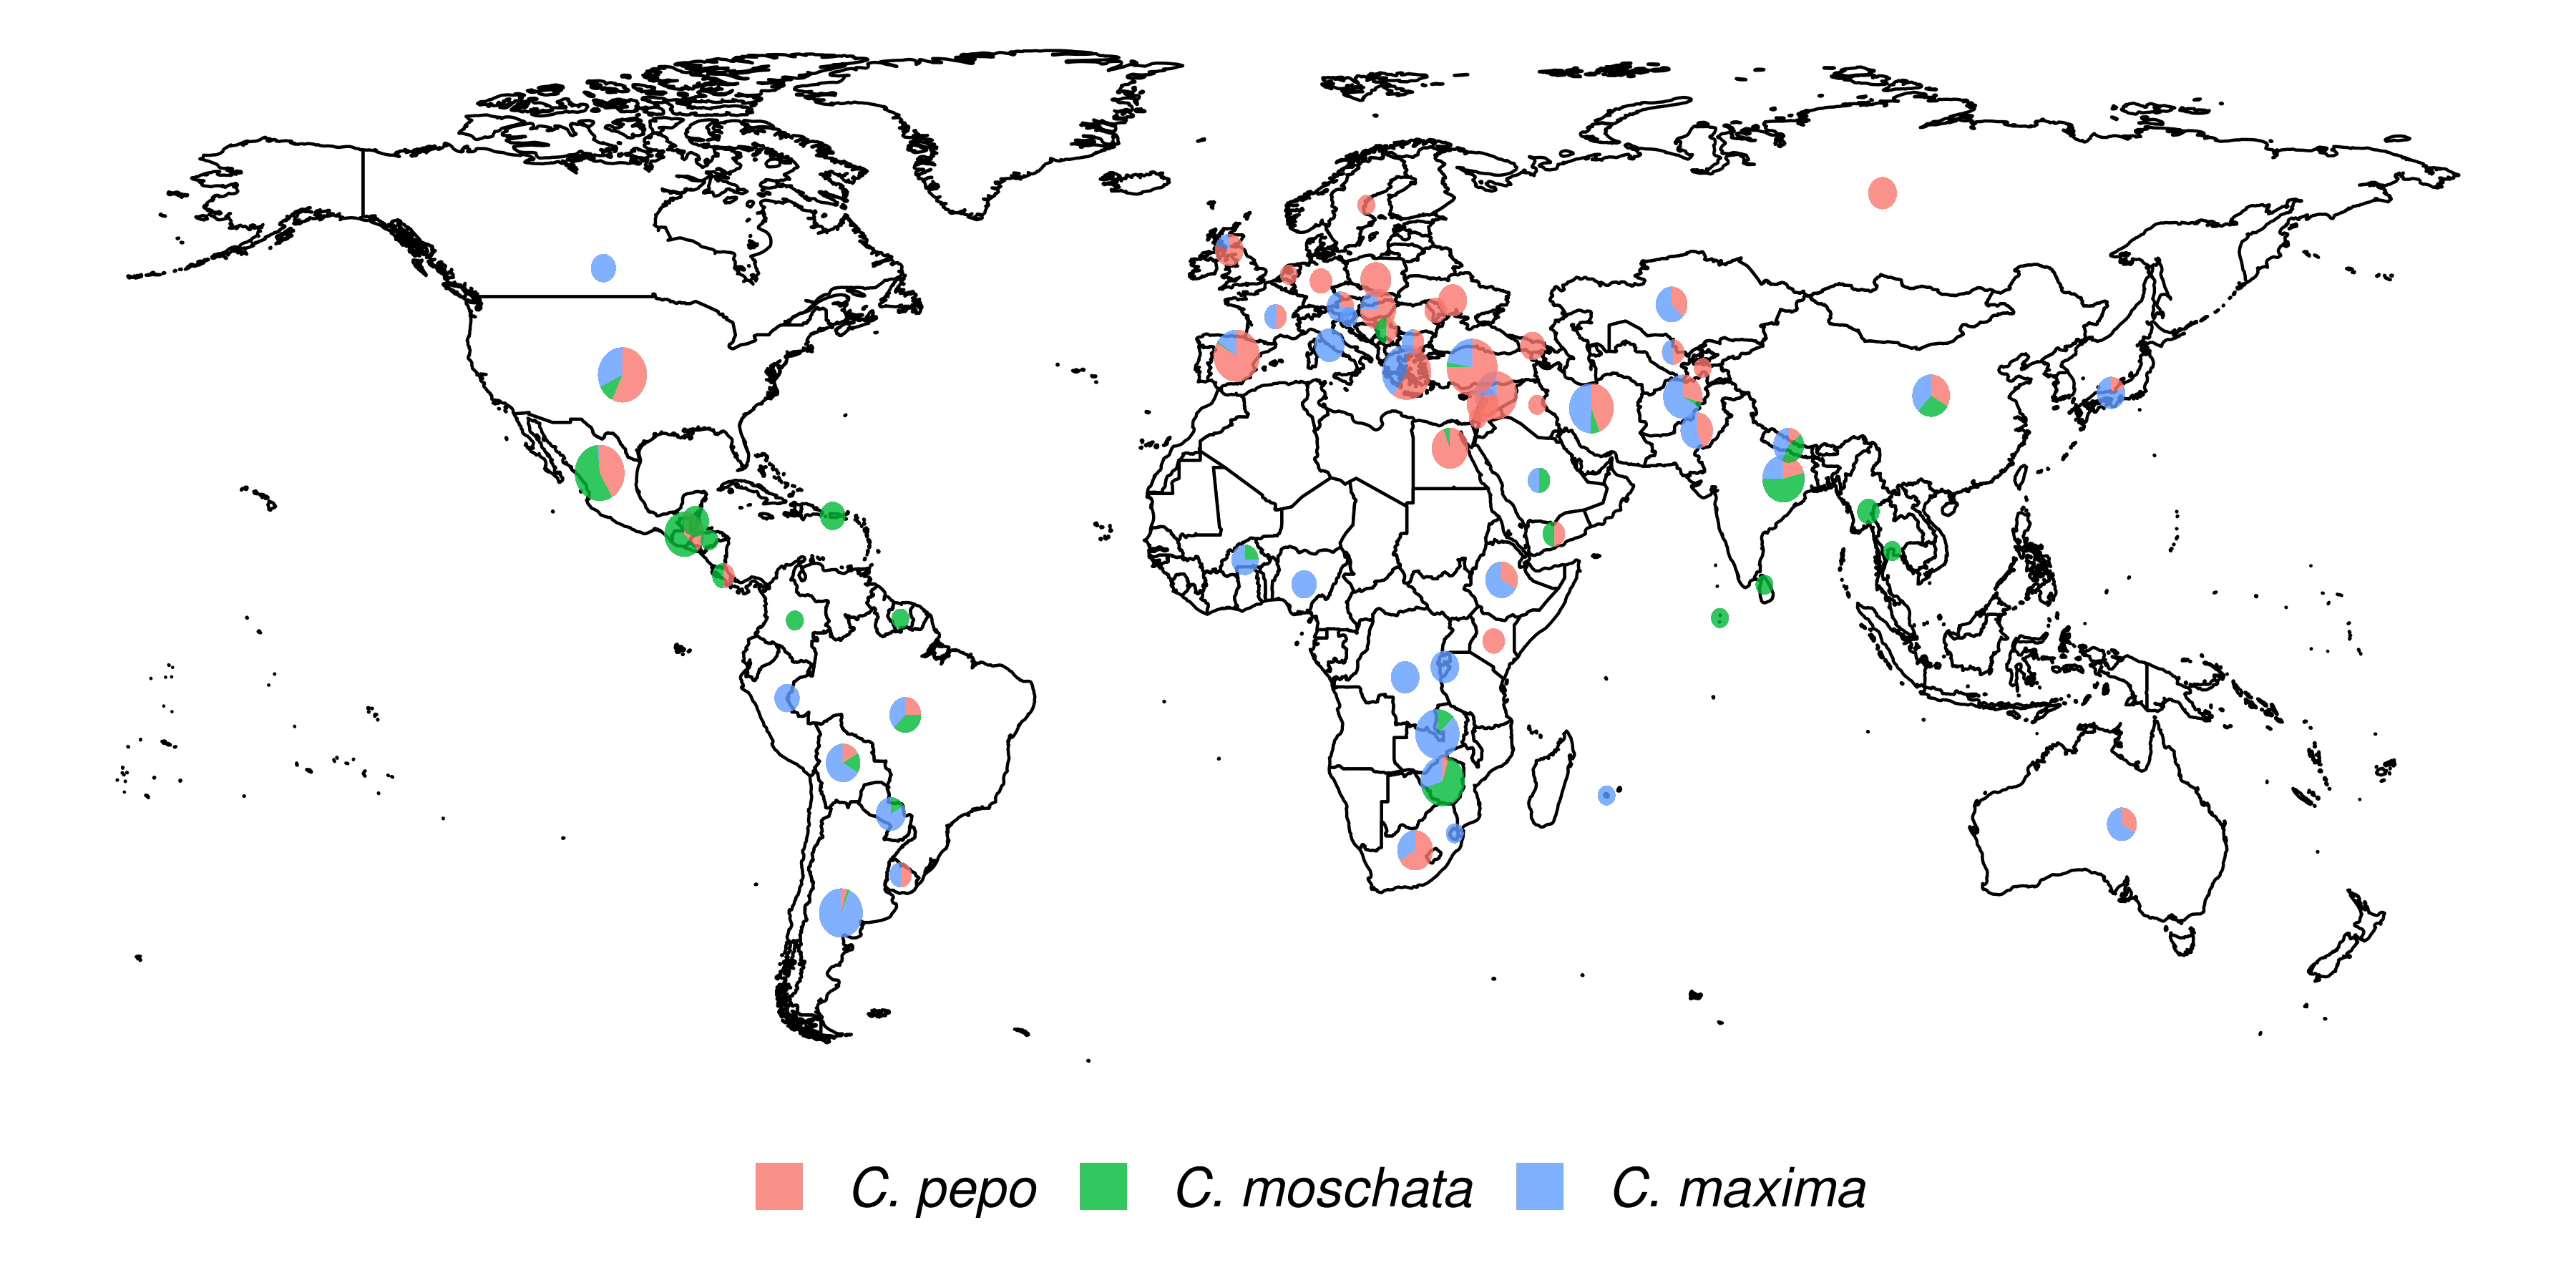
\includegraphics[width=\textwidth]{../final_figures/01_fig.png}
	\end{center}
	\caption{Geographical distribution of the USDA \textit{Cucurbita} ssp. collection. The size of the pie chart is scaled according to the number of accessions. Sector areas correspond to the proportion of the three species. \label{fig:1}}
\end{figure}

\clearpage


\begin{figure}[h]
	\begin{center}
		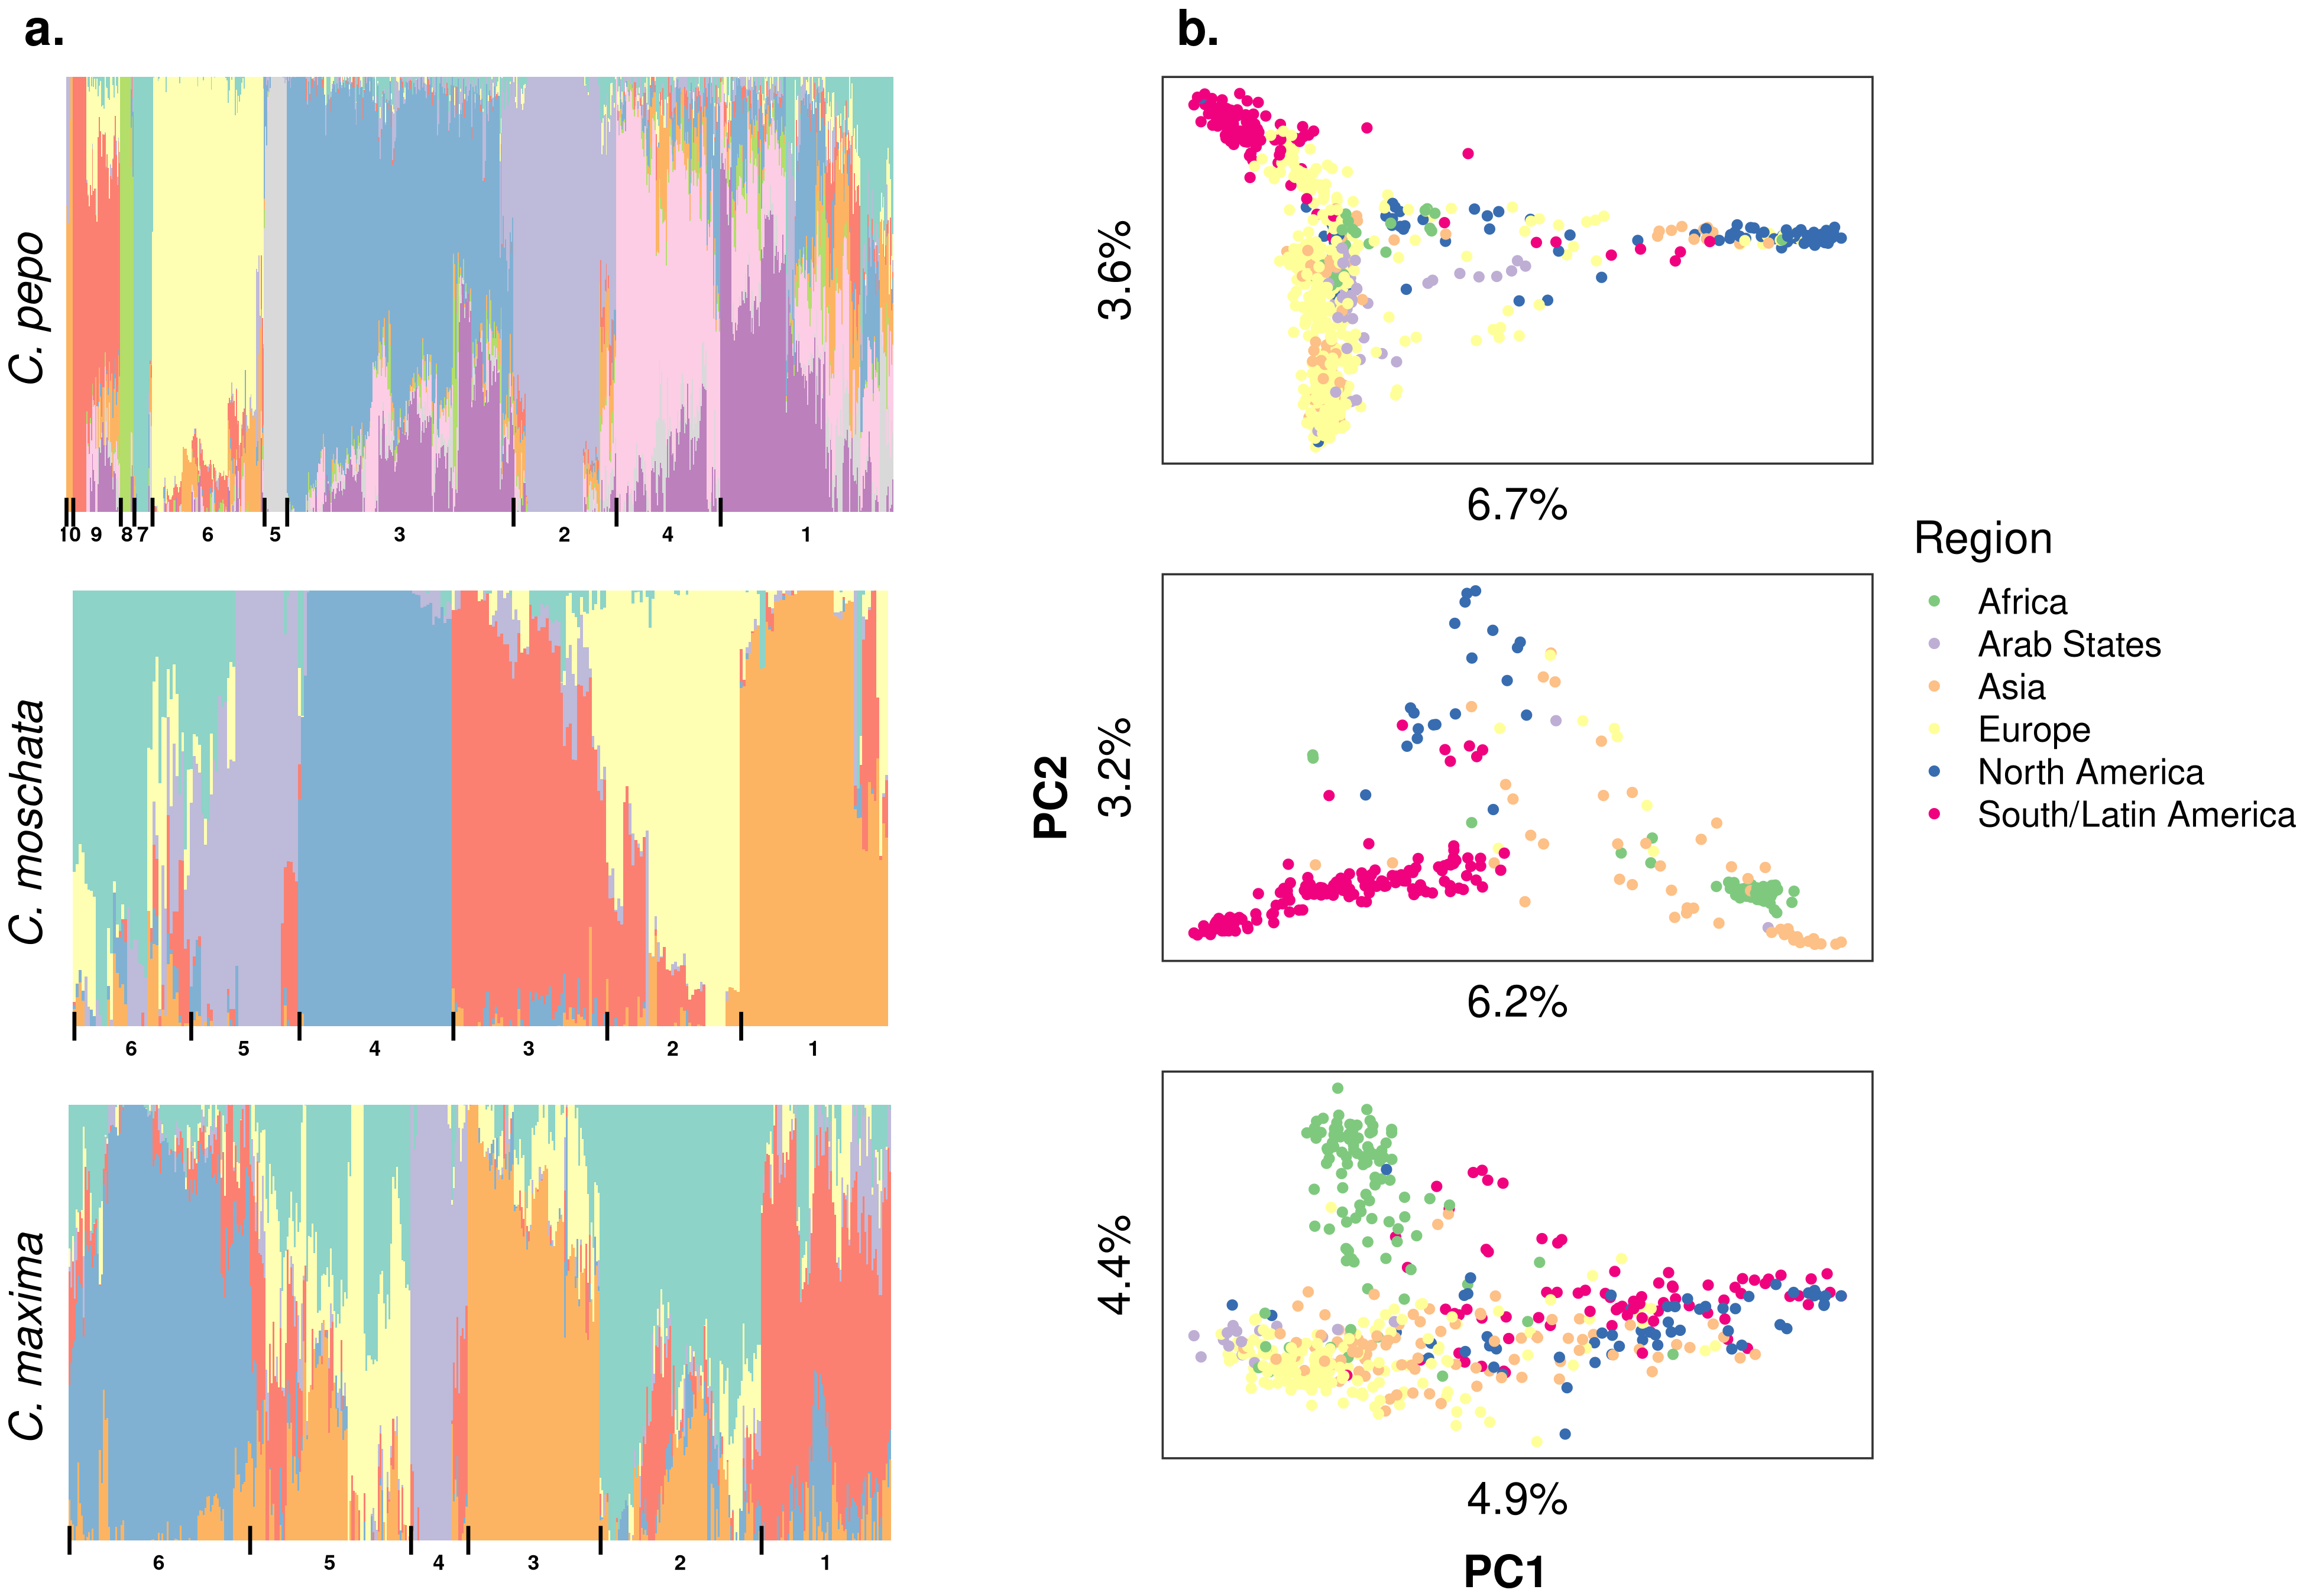
\includegraphics[width=\textwidth]{../final_figures/03_fig.png}
	\end{center}
	\caption{Population structure results aligned vertically by species. \textbf{Panel a.} Admixture plots: each stacked barplot represents an accession colored by proportion of inferred ancestral population. Groups based on hierarchical clustering are delimited by vertical bars and labeled with numbers along the bottom. \textbf{Panel b.} Plots of the first two principal components (PC) of accessions colored by region, variation explained by PCs is labeled on each axis. \label{fig:3}}
\end{figure}

\clearpage

\begin{figure}[h]
	\begin{center}
		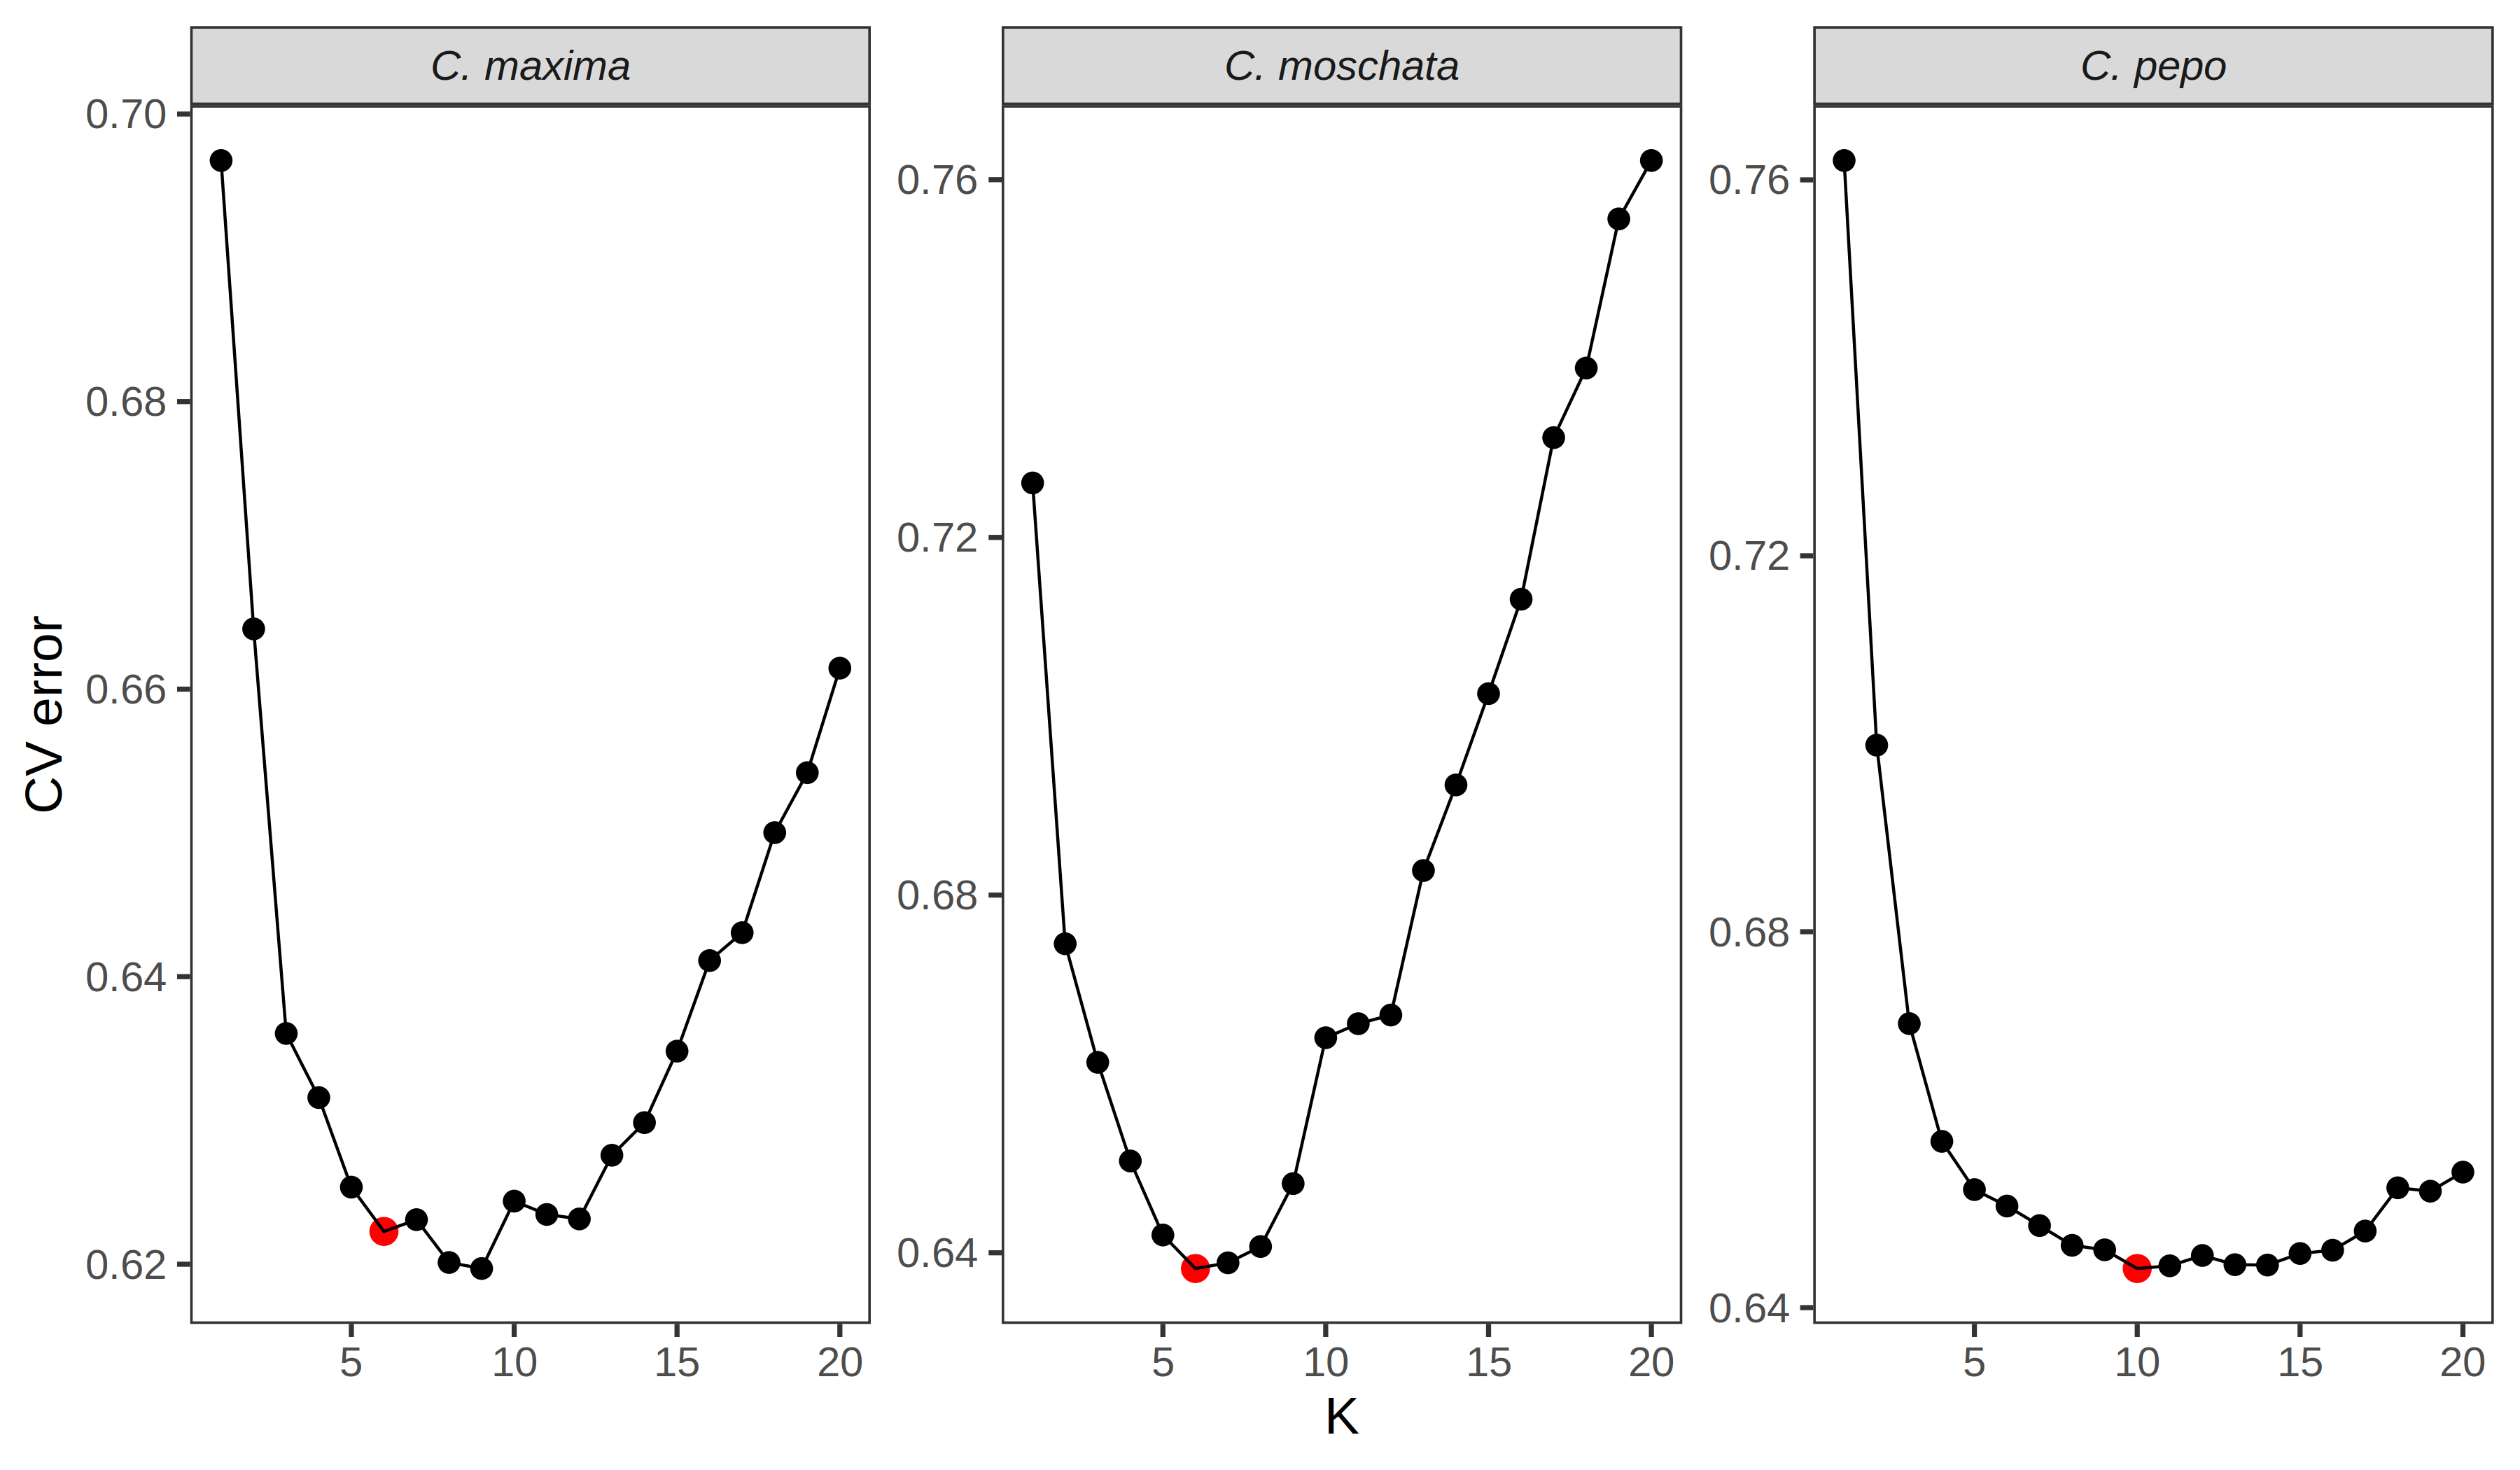
\includegraphics[width=\textwidth]{../final_figures/04_fig.png}
	\end{center}
	\caption{Cross-validation error plots used to pick the optimum $k$ value for admixture analysis. The $k$ value that balances minimizing cross-validation error and parsimony was chosen for the final analysis. The chosen $k$ is labeled with a red point. \label{fig:4}}
\end{figure}

\clearpage

\begin{figure}[h]
	\begin{center}
		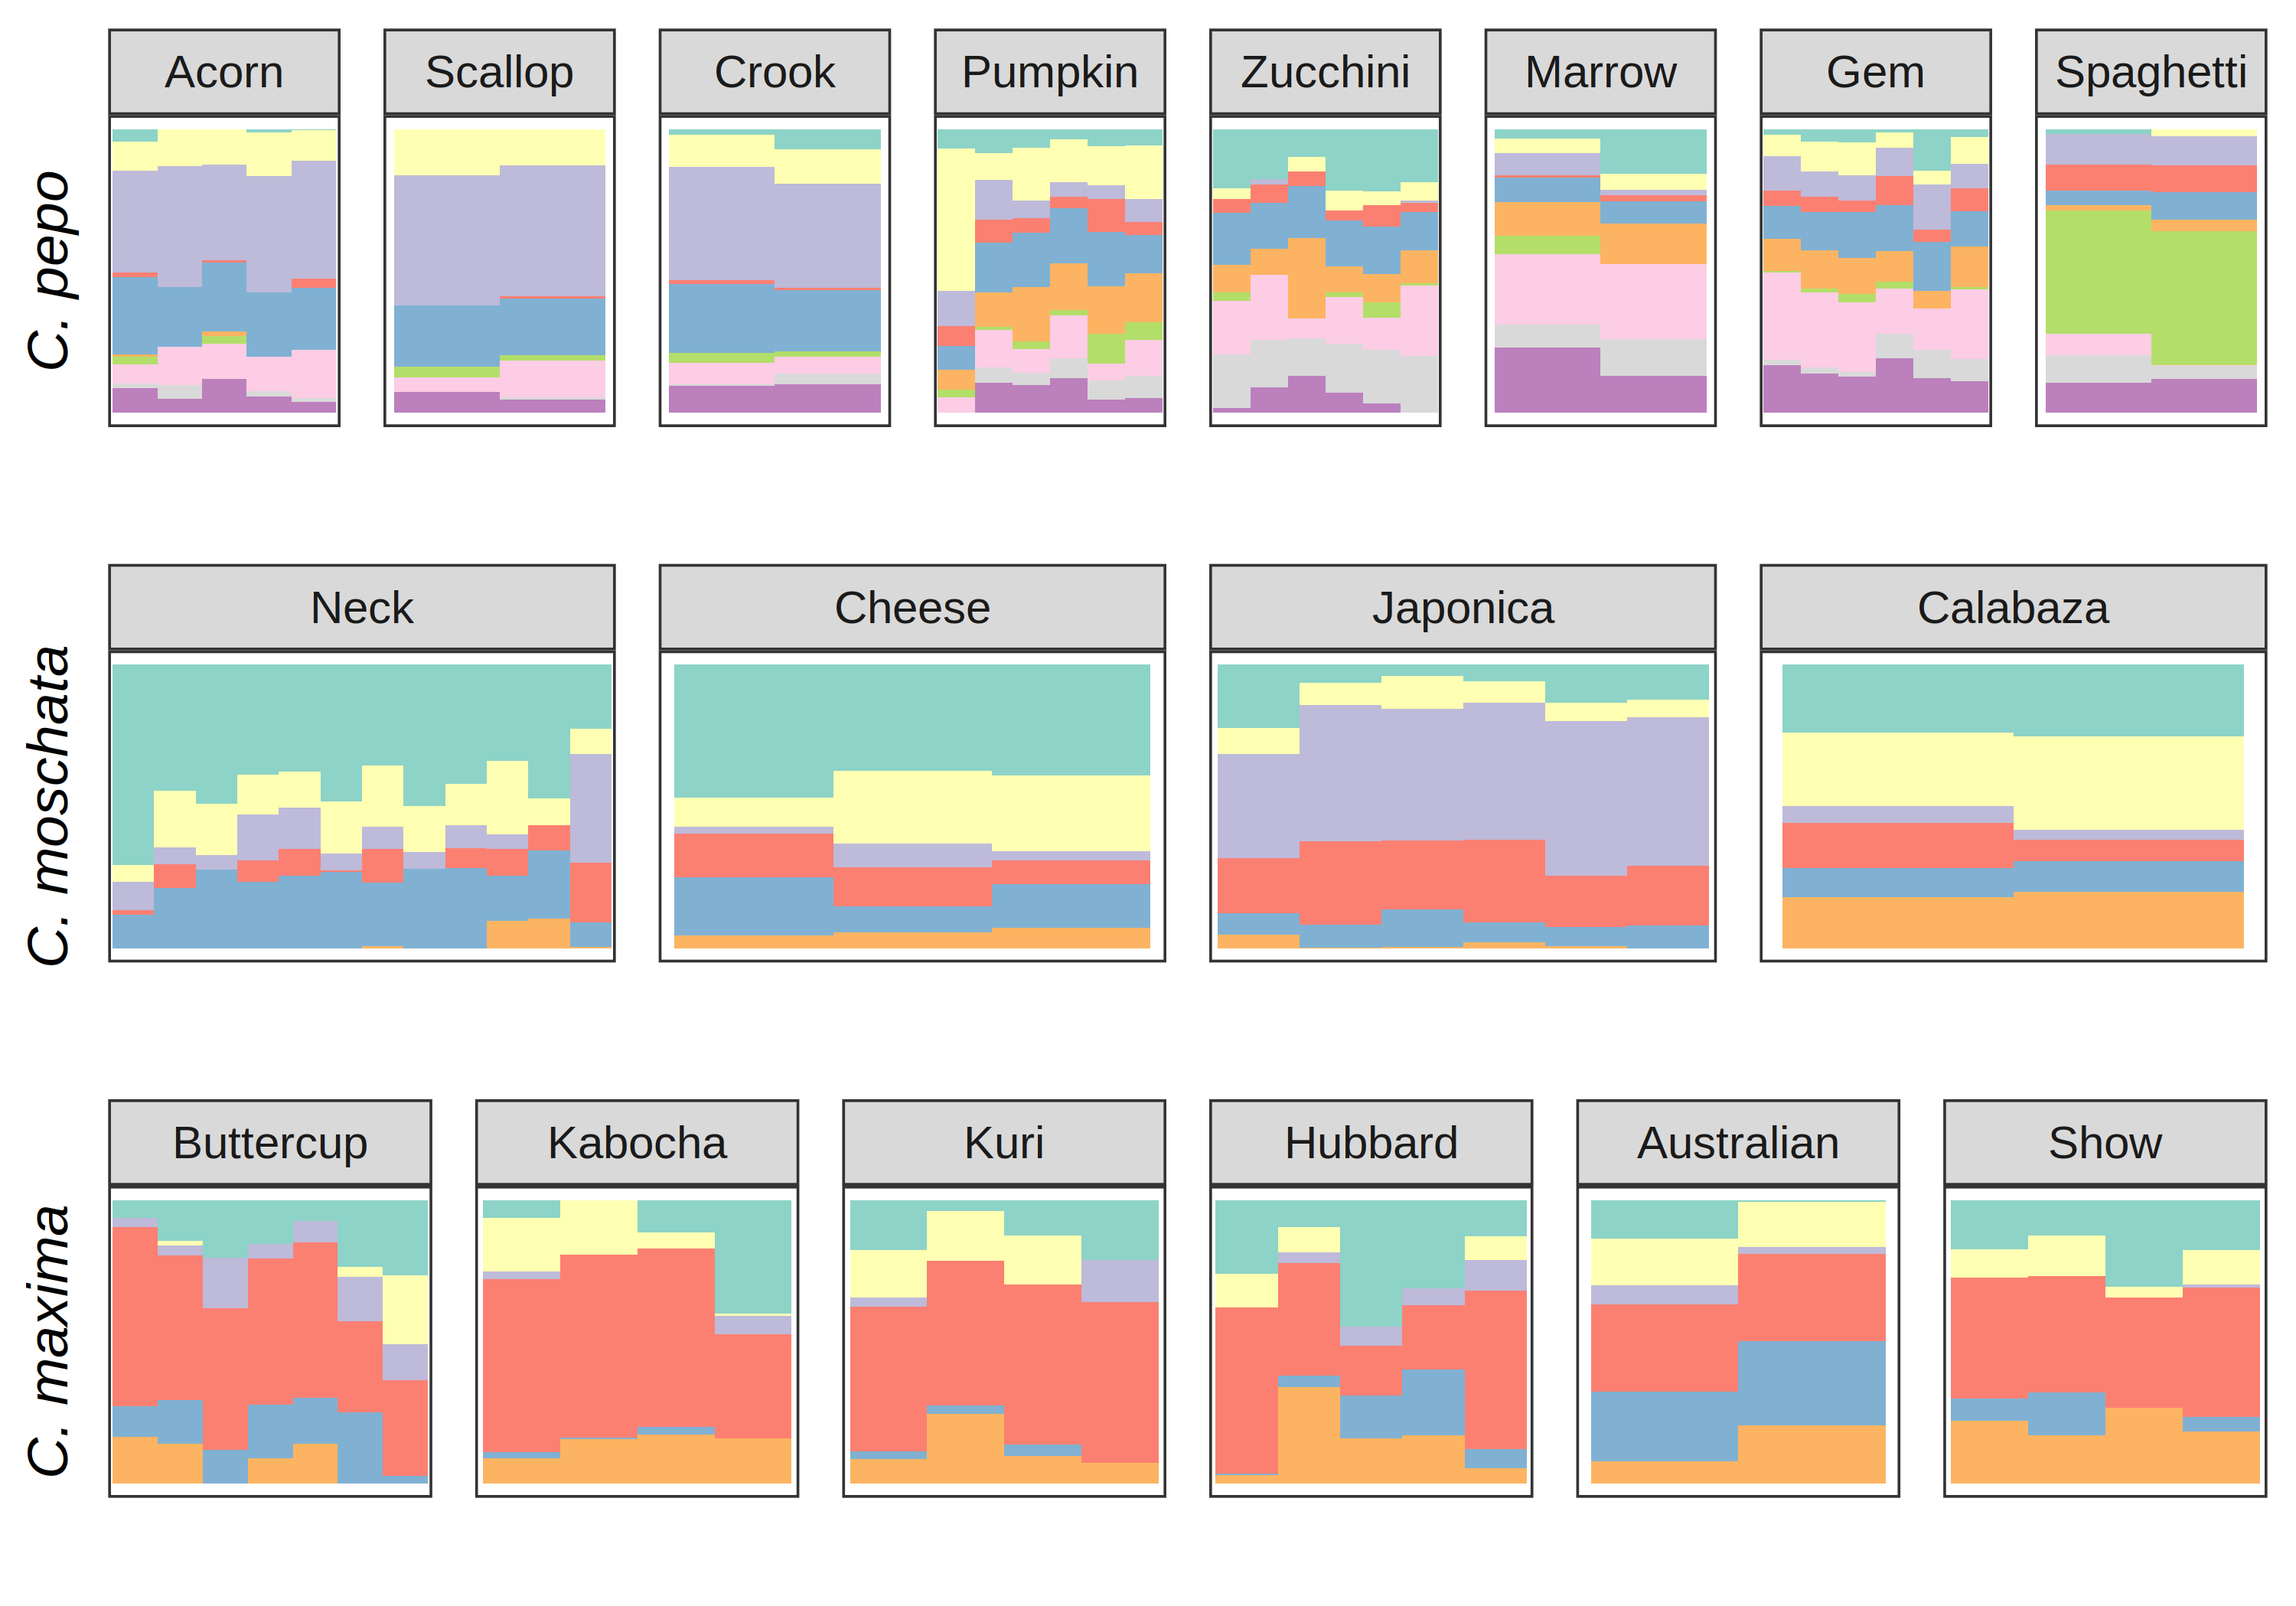
\includegraphics[width=\textwidth]{../final_figures/05_fig.png}
	\end{center}
	\caption{Ancestry coefficients projected on cultivars from each species. Results are shown grouped by market/varietal class. Colors correspond to the groups in Figure 3a. \label{fig:5}}
\end{figure}

\clearpage

\begin{figure}[h]
	\begin{center}
		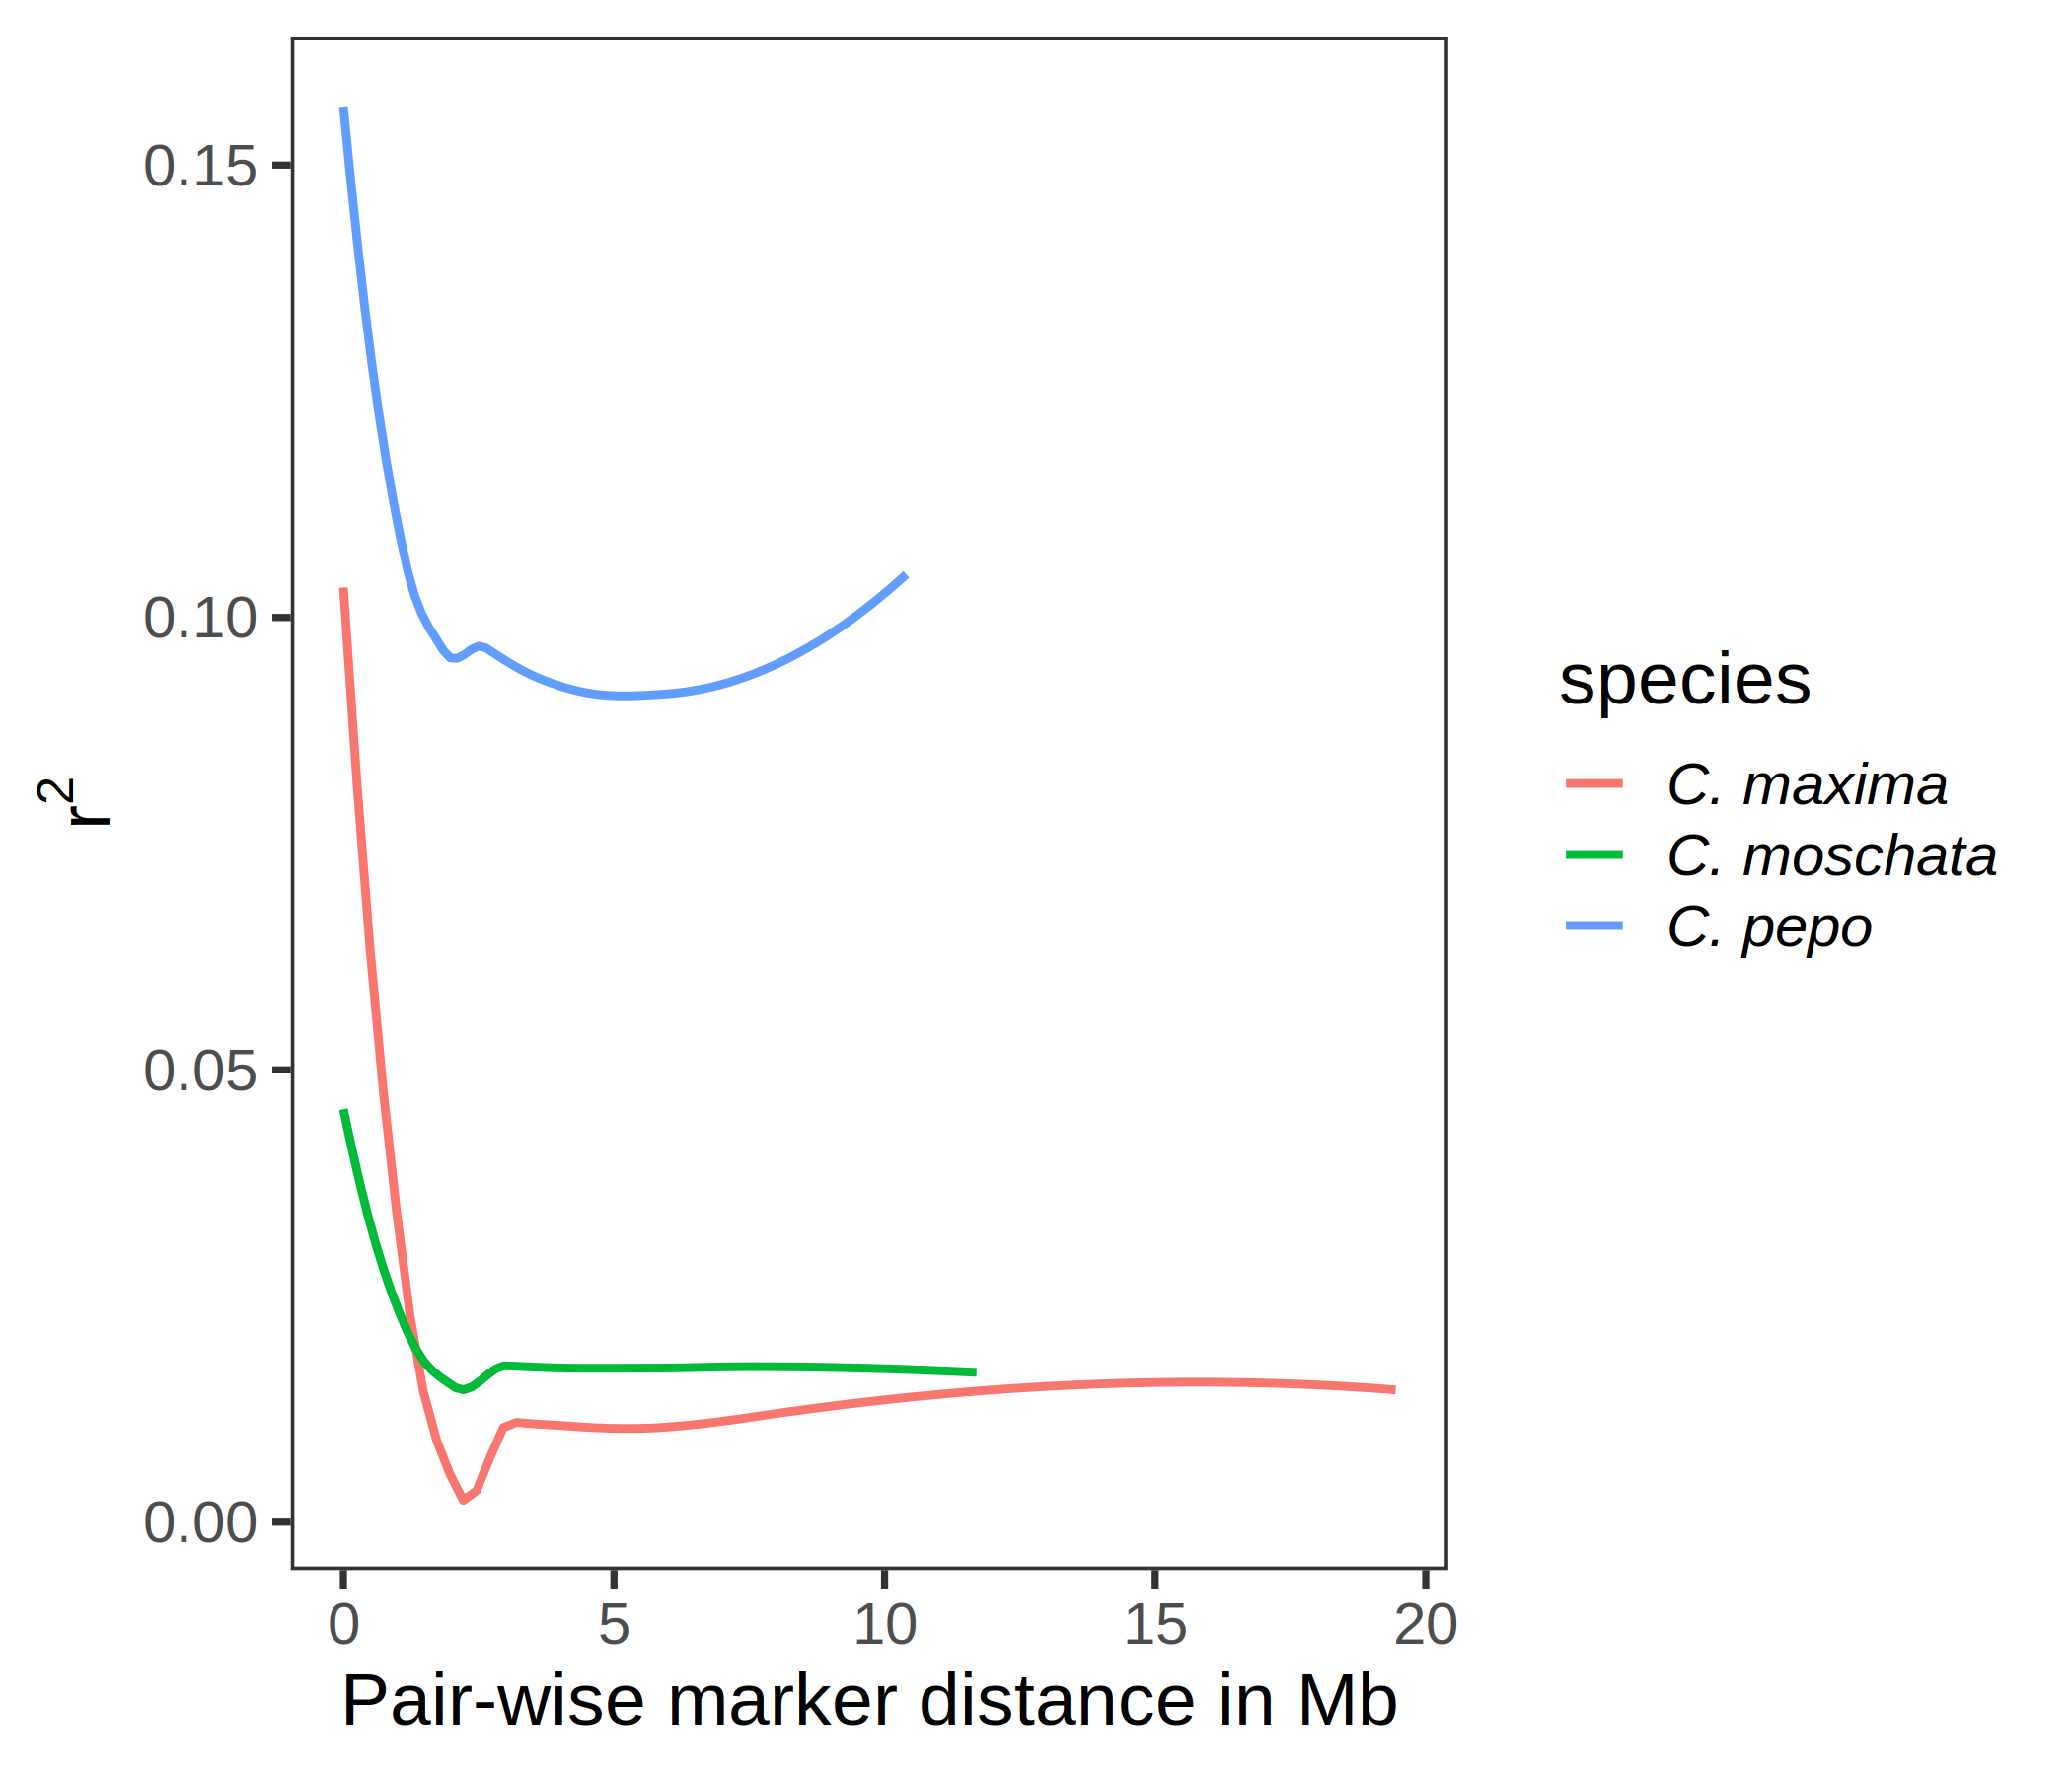
\includegraphics[width=0.8\textwidth]{../final_figures/06_fig.png}
	\end{center}
	\caption{Curves showing $r^{2}$ value as a measure of LD on the y-axis and pair-wise distance between markers in megabases on the x-axis. \label{fig:6}}
\end{figure}

\clearpage

\begin{figure}[h]
	\begin{center}
		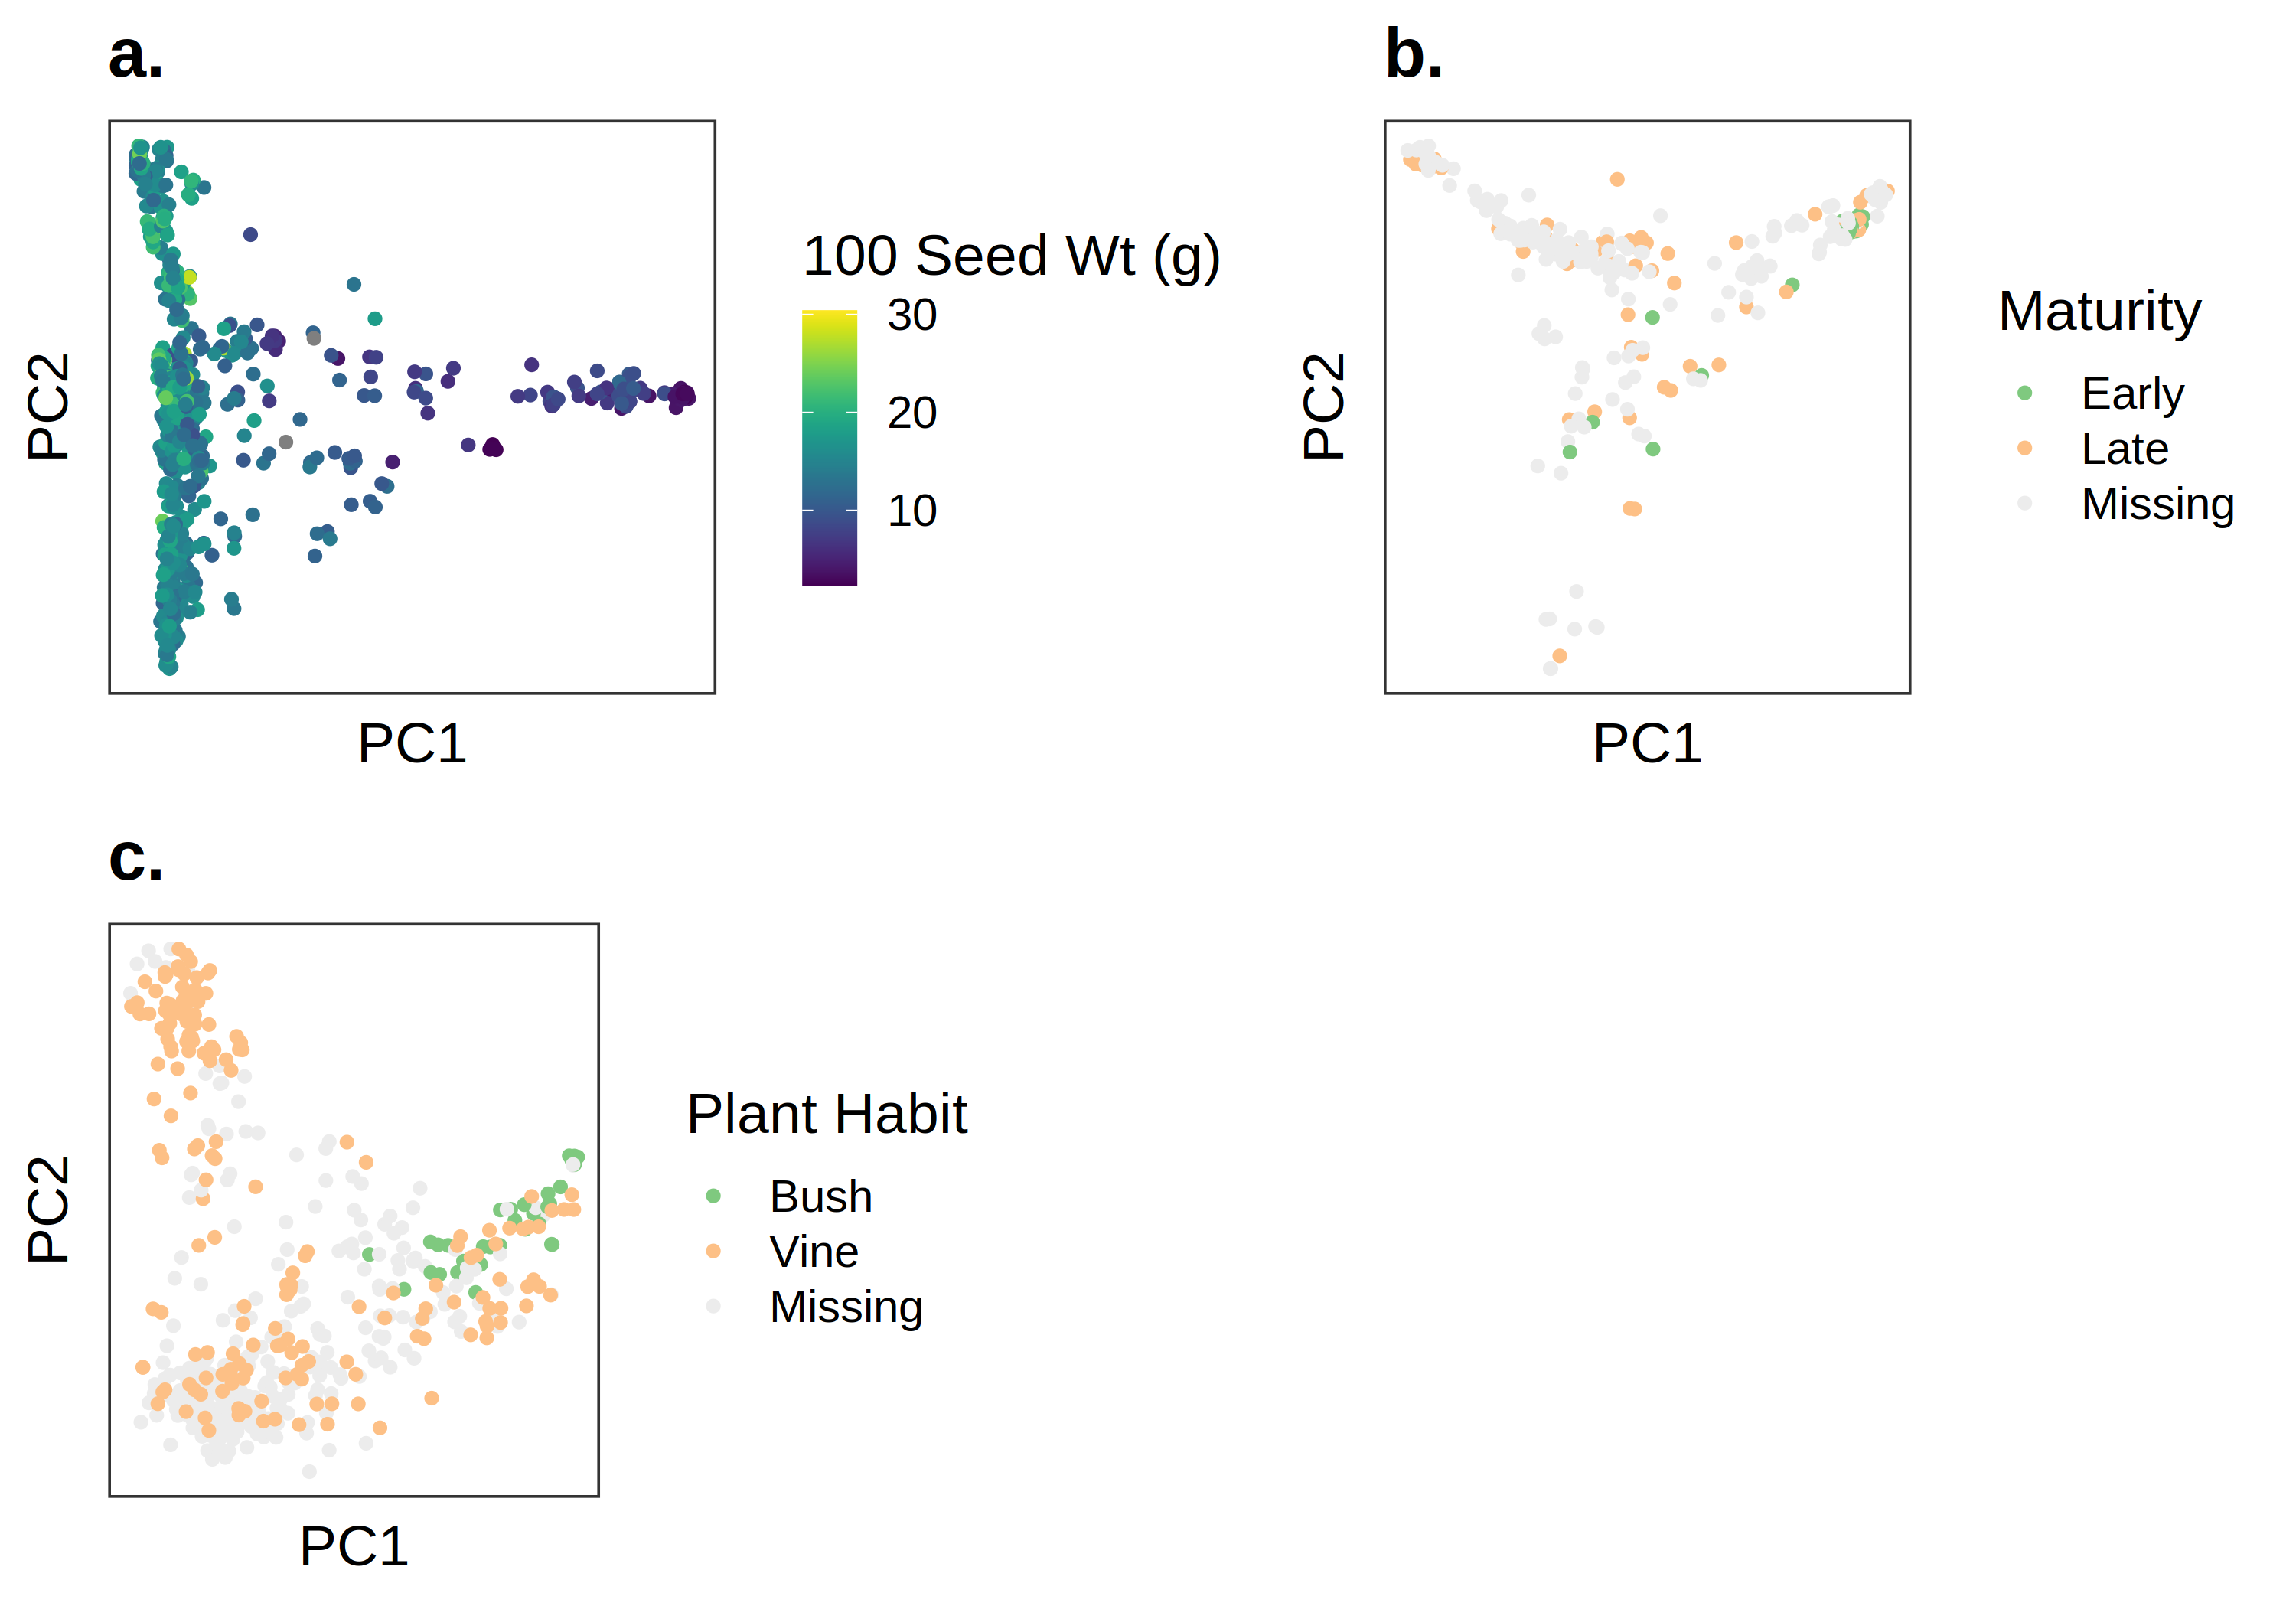
\includegraphics[width=0.8\textwidth]{../final_figures/07_fig.png}
	\end{center}
	\caption{ PCA plots with phenotypes superimposed over them for: \textbf{Panel a.}  100 seed weight in \textit{C. pepo}; { \color{red} \textbf{Panel b.} }maturity in \textit{C. moschata}; \textbf{Panel c.} plant habit in \textit{C. maxima}.\label{fig:7}}
\end{figure}

\clearpage

\begin{figure}[h]
	\begin{center}
		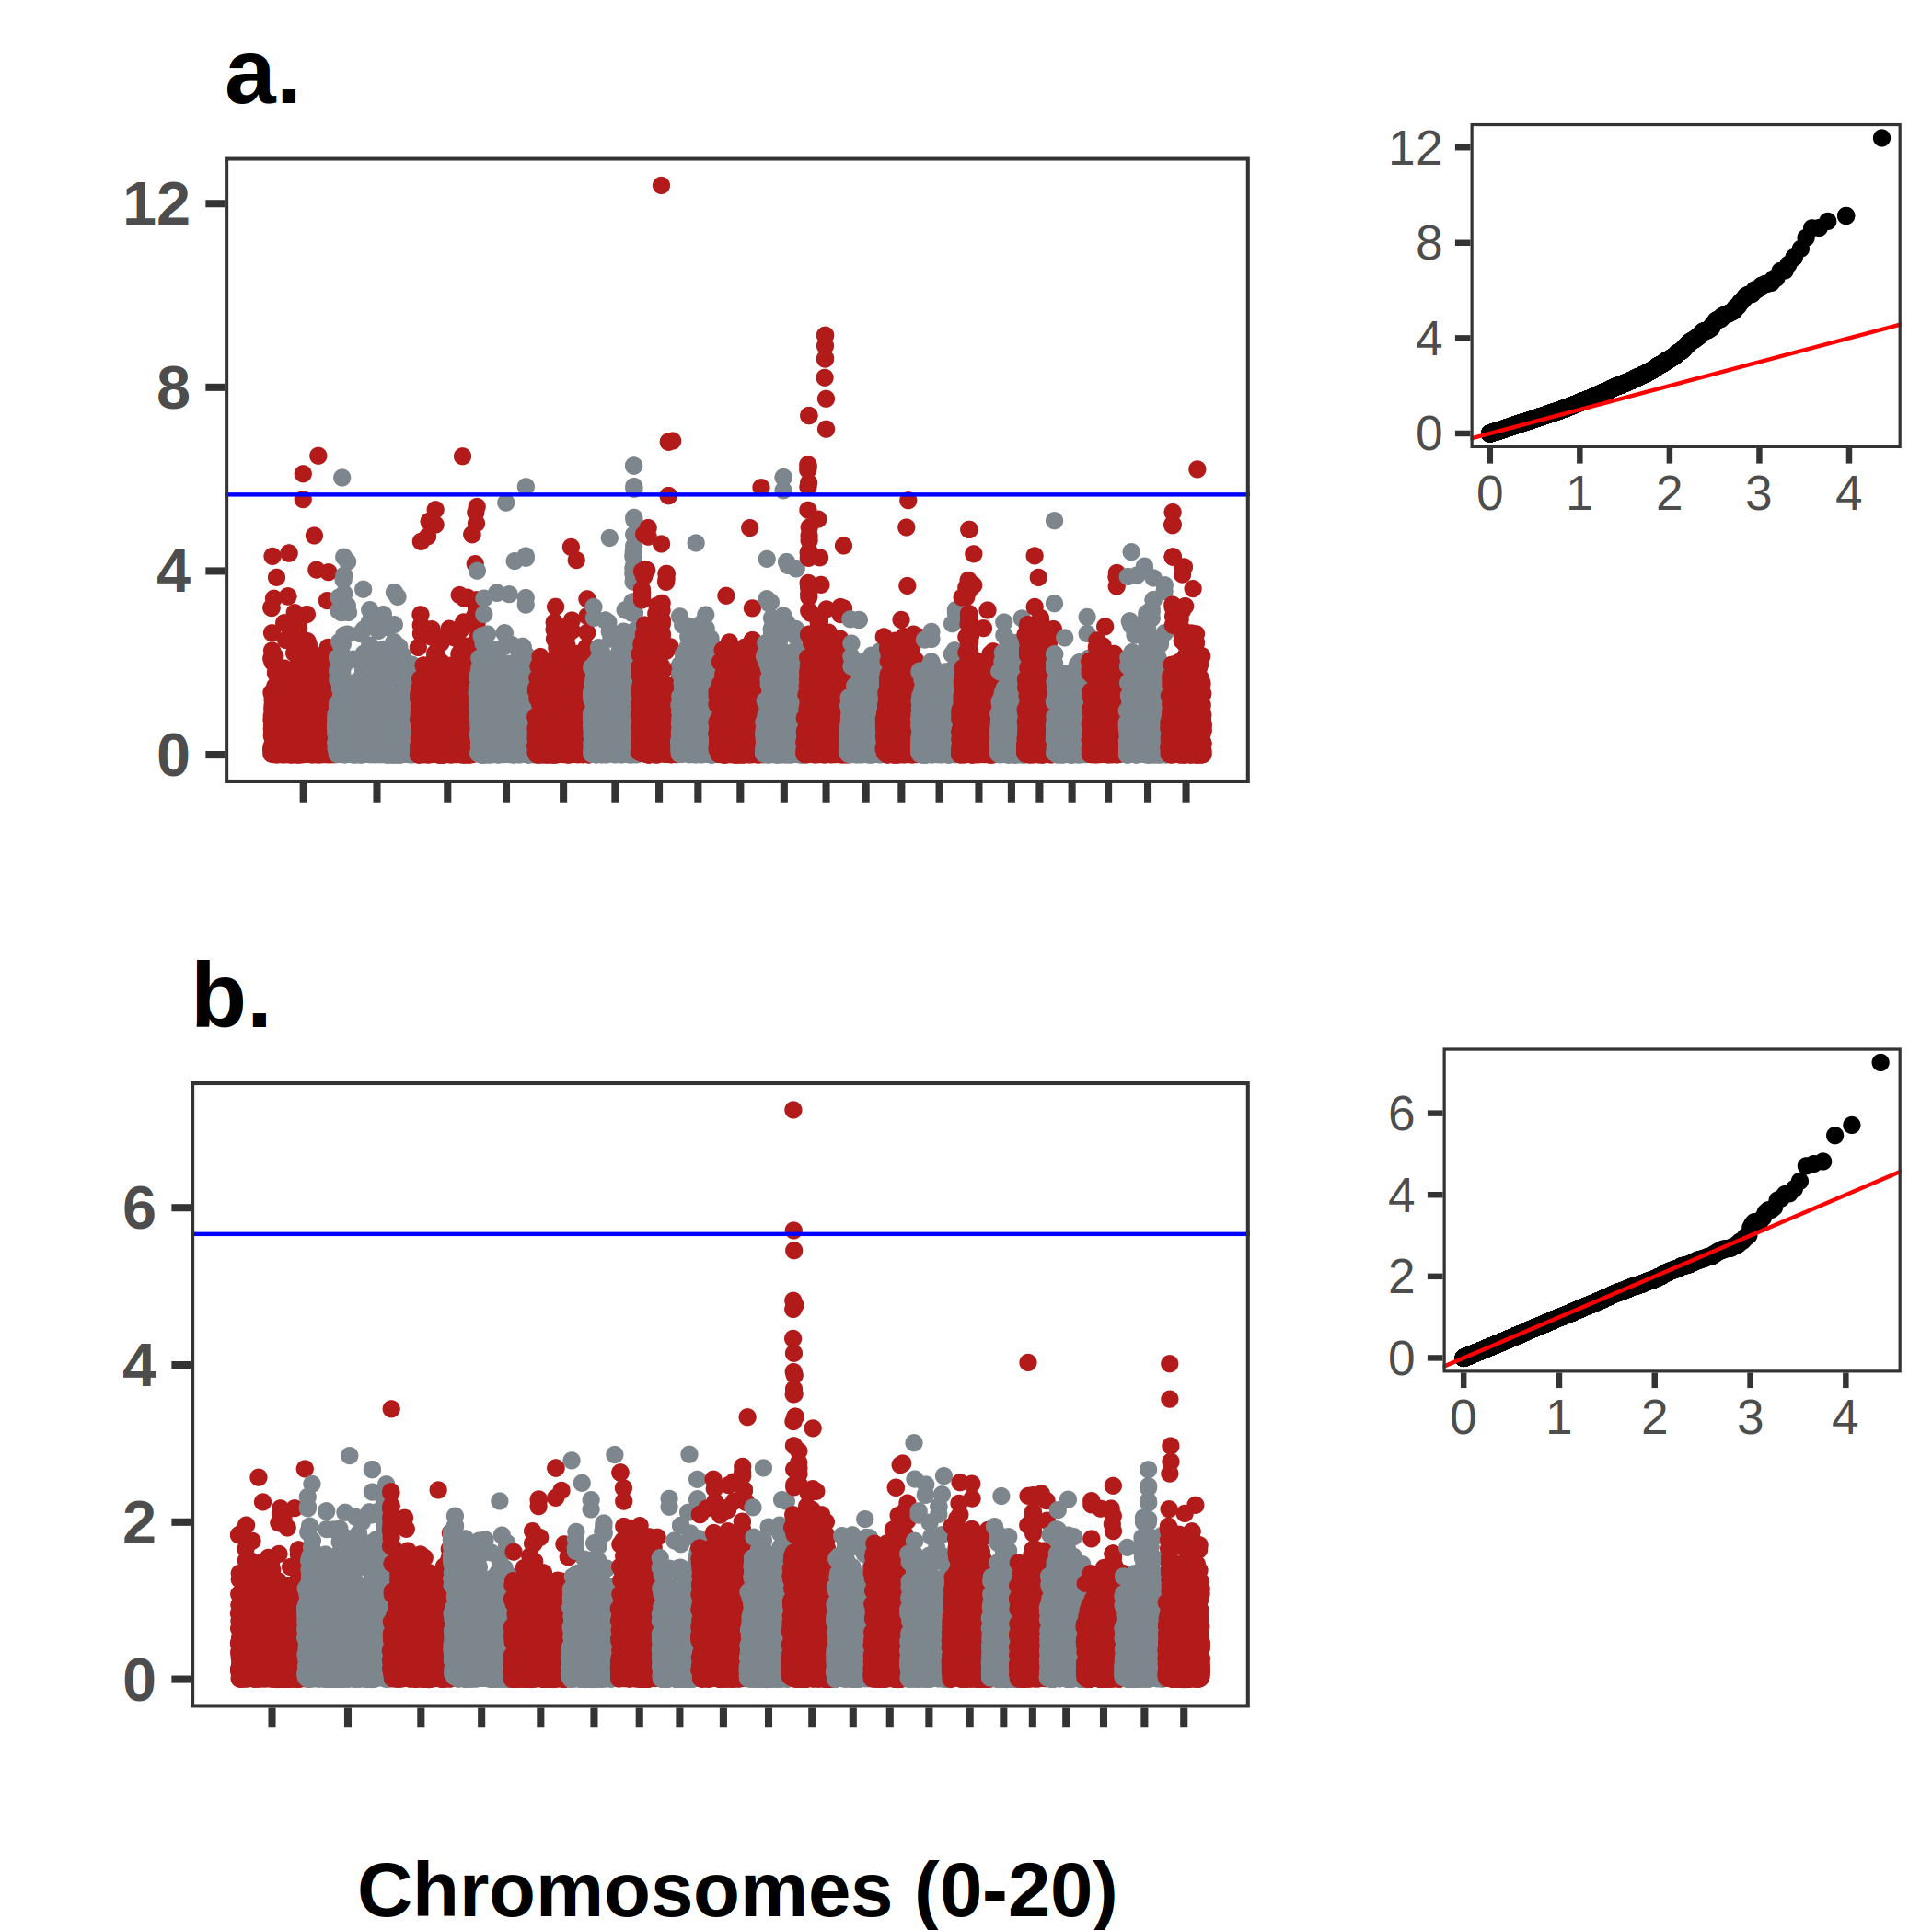
\includegraphics[width=0.6\textwidth]{../final_figures/08_fig.png}
	\end{center}
	\caption{GWAS results for the \textit{Bu} gene in \textit{C. pepo}. \textbf{Panel a.} shows the association results using the historical data with accompanying Q-Q plot. \textbf{Panel b.} shows the results using the contemporary data set. Both analyses supported an association on chromosome 10. \label{fig:8}}
\end{figure}

\clearpage

\begin{figure}[h]
	\begin{center}
		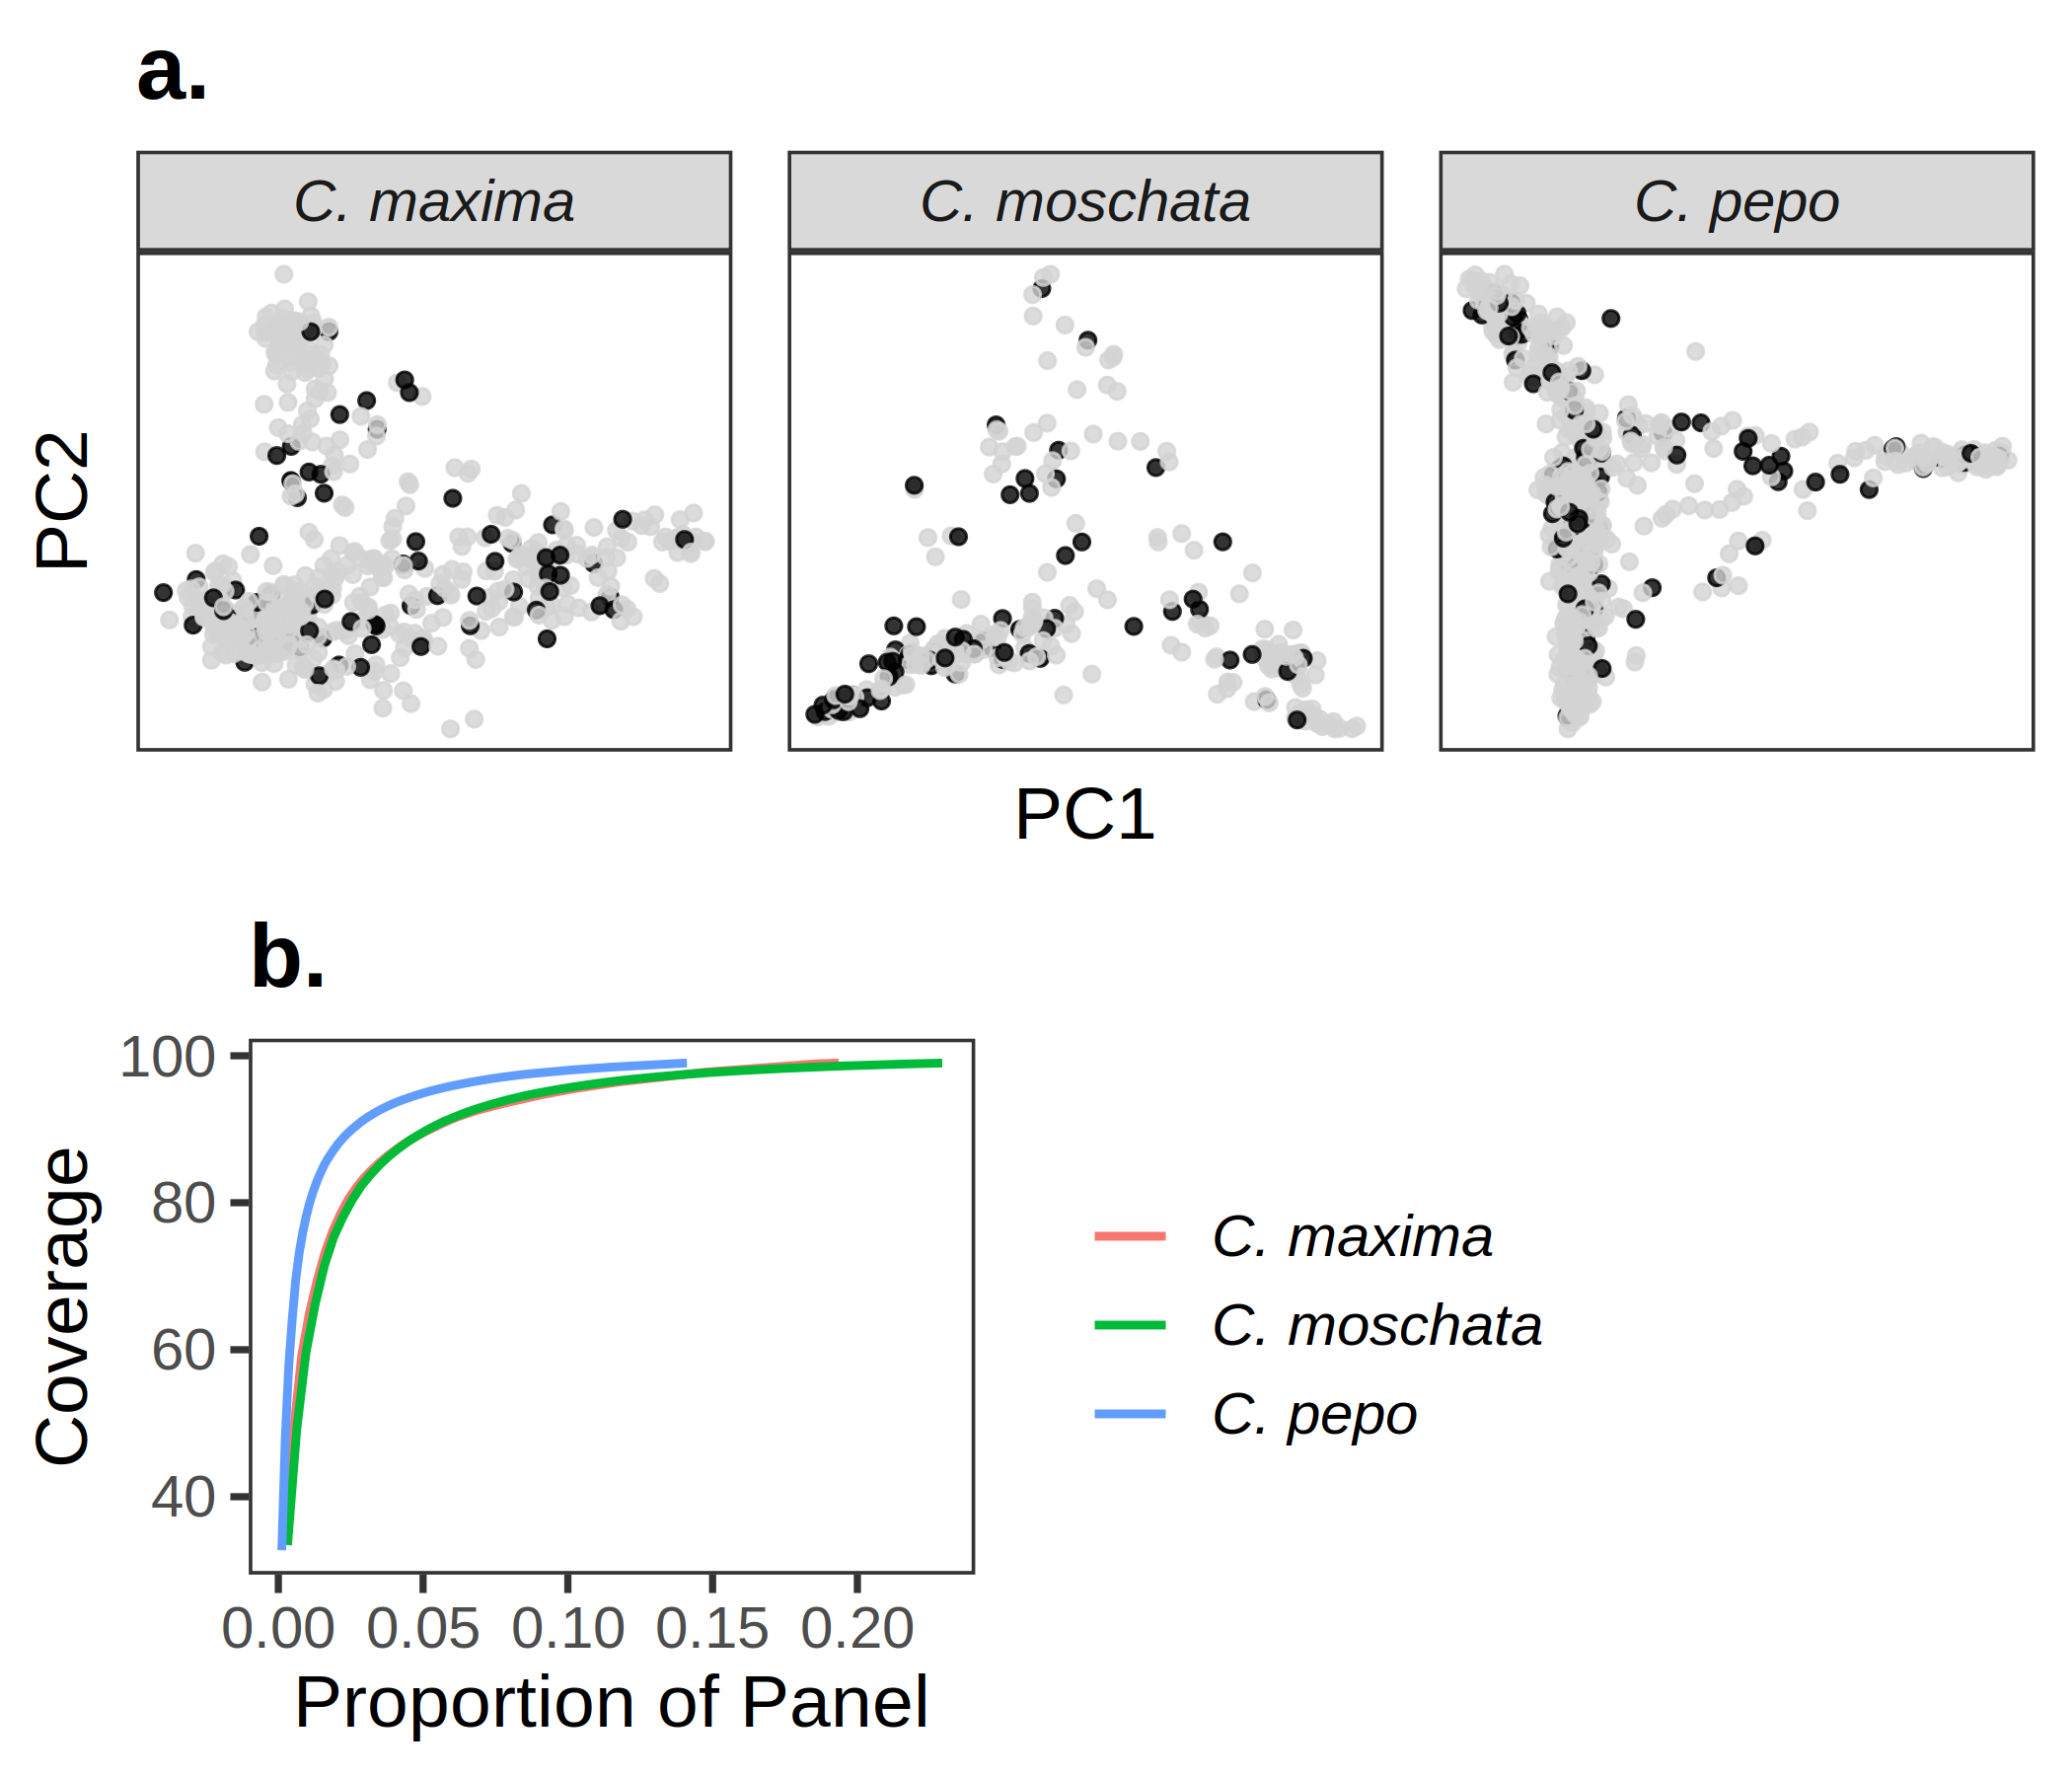
\includegraphics[width=0.8\textwidth]{../final_figures/09_fig.png}
	\end{center}
	\caption{Results from running GenoCore in each of the panels. {\color{red}\textbf{Panel a.}} shows the PCA plots for each panel with accessions selected by GenoCore represented as black points. {\color{red}\textbf{Panel b.}} shows the proportion of total accessions needed to obtain a certain coverage of diversity \label{fig:9}}
\end{figure}




%%% If you don't add the figures in the LaTeX files, please upload them when submitting the article.
%%% Frontiers will add the figures at the end of the provisional pdf automatically
%%% The use of LaTeX coding to draw Diagrams/Figures/Structures should be avoided. They should be external callouts including graphics.
\clearpage

\section*{Tables}

\begin{table}[h]
	\begin{center}
\begin{tabular}{c c c c c c c}
	\hline
	& \multicolumn{2}{c}{\textbf{\textit{C. pepo}}} & \multicolumn{2}{c}{\textbf{\textit{C. moschata}}}& \multicolumn{2}{c}{\textbf{\textit{C. maxima}}} \\
	\hline
	\textbf{Chromosome} & \textbf{Raw} & \textbf{Filtered} & \textbf{Raw} & \textbf{Filtered} & \textbf{Raw} & \textbf{Filtered} \\
	\hline
	0 & 12498 & 2550 & 2708 & 546 & 1501 & 132 \\
	1 & 7497 & 2831 & 3890 & 1468 & 4185 & 121 \\
	2 & 5153 & 2049 & 3661 & 1538 & 2101 & 55 \\
	3 & 4875 & 1943 & 3472 & 1499 & 2201 & 51 \\
	4 & 4598 & 1982 & 6880 & 2553 & 5703 & 106 \\
	5 & 4045 & 1628 & 2716 & 887 & 3115 & 46 \\
	6 & 3871 & 1384 & 3262 & 1159 & 3035 & 92 \\
	7 & 3129 & 1222 & 2668 & 969 & 2705 & 62 \\
	8 & 3875 & 1583 & 2348 & 810 & 2391 & 61 \\
	9 & 3766 & 1390 & 3106 & 995 & 2750 & 84 \\
	10 & 3585 & 1488 & 3550 & 1327 & 2297 & 52 \\
	11 & 3227 & 1216 & 4336 & 1830 & 3713 & 131 \\
	12 & 3089 & 1163 & 3711 & 1330 & 2026 & 47 \\
	13 & 3434 & 1350 & 3106 & 1280 & 2131 & 82 \\
	14 & 3543 & 1291 & 4753 & 1929 & 4317 & 100 \\
	15 & 2640 & 960 & 3564 & 1321 & 2662 & 58 \\
	16 & 3088 & 1060 & 2933 & 1107 & 2058 & 100 \\
	17 & 2994 & 1175 & 2885 & 1096 & 2195 & 86 \\
	18 & 3053 & 1258 & 3341 & 1316 & 1826 & 46 \\
	19 & 3381 & 1340 & 2638 & 990 & 1793 & 46 \\
	20 & 3096 & 1155 & 2497 & 903 & 1893 & 41 \\
	\hline
	\textbf{Total} & \textbf{88437} & \textbf{32018} & \textbf{72025} & 2\textbf{6853} & \textbf{56598} & \textbf{1599} \\
	\hline
\end{tabular}
	\caption{Distribution and number of raw and filtered SNPs per chromosome for each species \label{tbl:1}}
	\end{center}
\end{table}

\clearpage

\begin{table}[h]
	\begin{center}
	\begin{tabular}{c p{5cm} p{5cm} p{5cm}}
		\hline
& \textbf{\emph{C. pepo}} & \textbf{\emph{C. moschata}} & \textbf{\emph{C. maxima}} \\
\hline
1 & Mixed Group; Many from Spain, Turkey, and Syria & Mostly from Mexico & Mixed; Primarily from South America and Asia \\
2 & Wild subsp. \emph{ovifera} var. \emph{texana} and var. \emph{ozarkana}; North American & Mostly Mexico and Guatemala & Mixed; Primarily from Asia and Europe \\
3 & Majority from Turkey & Mostly from Mexico & Mostly from North Macedonia \\
4 & Majority from North Macedonia & Mostly from Africa & Mostly from Argentina \\
5 & Majority from Egypt & Mostly from India & Mostly Turkey, Iran, Afghanistan \\
6 & Majority from Mexico & Mixed origin Europe and Americas;Many similar to cheese or neck type & Mostly from Africa \\
7 & Majority from Syria & & \\
8 & Majority from Pakistan and Afghanistan & & \\
9 & Majority from Spain & & \\
10 & Wild subsp. \emph{fraterna}; Central American & & \\
\hline
	\end{tabular}
	\caption{Commonalities among accessions in each group, most groupings are dictated by geography \label{tbl:2}}
	\end{center}
\end{table}

\clearpage

\begin{center}
\begin{longtable}{l l l l p{5cm} c}
\hline
\textbf{Species} & \textbf{Trait} & $\mathbf{N}$ &\textbf{Type} & \textbf{Description} & $\mathbf{h_{G}^{2}}$ \\
\hline
\textbf{\emph{C. pepo}} & & & & & \\
& seed\_wt & 827 &Quantitative & Weight of 100 seeds in grams& 0.95 \\
& plant\_type & 404 &Binary & Historical plant architecture data coded as vining or bush& NA \\
& plant\_type2 & 292 &Binary & Contemporary plant architecture data coded as vining or bush& NA\\
& max\_vig & 413 & Ordinal & Maximum plant vigor on 1-5 scale& 0.588 \\
& min\_vig & 414 &Ordinal & Minimum plant vigor on 1-5 scale & 0.618 \\
& max\_width & 413 &Quantitative & Maximum fruit width in centimeters & 0.937 \\
& width\_min & 304 &Quantitative & Minimum fruit width in centimeters & 1\\
& len\_max & 413 &Quantitative & Maximum fruit length in centimeters & 0.748\\
& len\_min & 315 &Quantitative & Minimum fruit length in centimeters & 0.841\\
& flesh\_max & 421 &Ordinal & Maximum fruit thickness in centimeters & 0.614\\
& flesh\_min & 175 & Ordinal & Minimum fruit thickness in centimeters & 0.425\\
& sb\_nymph & 205 & Quantitative & Number of squash bug nymphs on plant & 0.181 \\
& sb\_adult & 249 &Quantitative & Number of adult squash bugs on plant & 0.206 \\
& cuc\_inj & 247 &Ordinal & Severity of beetle damage on a 0-4 scale & 0.228\\
& or\_flesh & 378 &Binary & Flesh color coded as orange or not orange & NA \\
& yl\_flesh & 378 &Binary & Flesh color coded as yellow or not yellow & NA \\
& yl\_fruit & 182 &Binary & Color of fruit coded as yellow or not yellow & NA\\
& tan\_fruit & 182 &Binary & Color of fruit coded as tan or not tan & NA \\
& gn\_fruit & 182 &Binary & Color of fruit coded as green or not green & NA \\
& globe\_fruit & 333 &Binary & Fruit shape as globe or not globe & NA\\
& oblong\_fruit & 333&Binary & Fruit shape as oblong or not oblong & NA\\
& smooth\_fruit & 130 &Binary & Furit texture as smooth or not smooth & NA\\
& rib\_fruit & 130 &Binary & Degree of ribbing & NA \\
& spec\_fruit & 248 &Binary & Fruit patterning as speckled or not speckled & NA \\
& mot\_fruit & 248 & Binary & Fuit patterning as mottled or not mottled & NA \\
& solid\_fruit & 248& Binary & Fruit patterning as solid color or patterned & NA \\
\textbf{\emph{C. moschata}} & && & &\\
& fruit\_len & 123&Quantitative & Fruit length in centimeters & 0.804 \\
& fruit\_diam &123 &Quantitative & Fruit diameter in centimeters & 0.478 \\
& maturity & 109&Binary & Fruit maturity as early or late & NA \\
& or\_fruit & 145&Binary & Fruit color coded as orange or not orange & NA \\
& smooth\_fruit & 130 &Binary & Fruit surface texture encoded as smooth or not smooth & NA \\
\textbf{\emph{C. maxima}}& & & & &\\
& len & 346 &Quantitative & Fruit length in centimeters & 0.374\\
& set & 350 &Ordinal & Fruit set from poor to excellent (1-9) & 0.254 \\
& diam & 345 &Quantitative & Fruit diameter in centimeters & 0.249 \\
& watermelon\_mosaic & 297 &Ordinal & Susceptibility to WMV from slight to severe (0-9) &  0.18\\
& cuc\_mosaic & 100 &Ordinal & Cucumber mosaic susceptibility from slight to severe (0-9) & 0.129 \\ 
& maturity & 329 &Quantitative & Number of days from field transplanting to date of first pollination & 0.388\\
& unif & 341 &Ordinal & Fruit uniformity from poor to excellent (1-9) & 0.157 \\
& pm & 287 &Ordinal & Susceptibility to PM from slight to severe (0-9) & 0.192\\
& plant\_habit & 352 &Binary & Plant type as vining or not vining& NA \\
& vig & 353 &Ordinal & Plant vigor from poor to excellent (1-9)& 0.066 \\
& or\_flesh & 288 &Binary & Flesh color as orange or not orange & NA \\
& rib & 338 &Ordinal & Fruit ribbing from slight to pronounced (1-9) & 0.427 \\
& fruit\_spot & 272 &Ordinal & Fruit spotting from slight to pronounced (1-9) & 0.132 \\
& gray\_fruit & 264 &Binary & Fruit color encoded as gray or not gray & NA \\
& or\_fruit & 264 &Binary & Fruit color encoded as orange or not orange & NA \\
& gn\_fruit & 264 &Binary & Fruit color encoded as green or not green & NA \\
\hline
	\caption{Descriptive data for each trait including trait type, number of data points for each trait, a brief trait description, and an estimate of genomic heritability {$h_{G}^{2}$} . \label{tbl:3}}
\end{longtable}
\end{center}

\end{document}
